%\section{Further Detailed Performance Analysis}%

\chapter{\rnn{} Performance}%
\label{sec:off_ana}

This section dedicates to more detailed assessments of the \rnn{} behavior 
\textcolor{red}{in the period 2017-2018 with respect to the previous electron trigger cut-based strategy.}
%with respect to the previous electron trigger strategy. 
Using \Zee{} \tnp{}
selection, we investigate the agreement between the two triggers and investigate
for possible biases caused by the introduction of the \rnn{} using the variables
employed by the likelihood algorithm. \textcolor{red}{Since} offline and final HLT electron
selection are based on such variables, limiting the evaluation to them suffice
to understand any possible impact of the \rnn{} algorithm in most analyses.
Additionally, these variables are interesting \textcolor{ref}{as} they compact the input space
in a set of few variables with low correlation (i.e., when compared to the ring
sums) and high interpretability power. One should keep in mind that the \rnn{}
algorithm had access only to the ring description during Run~2 operation.

As indicated in
Table~\ref{tab:quadrant_vs_agreement}, we perform two analyses evaluating the
trigger \textcolor{red}{performance} with and without \rnn{}, when applied to the tag (Agreement Analysis) and
to the probe (Quadrant Analysis).
\textcolor{red}{ It is worth reminding that Tag \& Probe events have one electron (probe) that was not used to decide the selection of that event at the trigger level.
}

\begin{table}[ht!]\footnotesize
\centering
\caption{Customized \Zee{} \tap{} selection criteria employed in the
agreement and quadrant analyses \textcolor{red}{in the Run 2 (2017-2018 period)}.}%
\label{tab:quadrant_vs_agreement}
\resizebox{\textwidth}{!}{%
  \begin{tabular}{p{2cm}p{4.5cm}p{5.5cm}}
\hline
\hline
\hline
& Agreement Analysis (Section~\ref{ssec:agreement}) & Quadrant Analysis
(Section~\ref{ssec:quadrant}) \\
\hline
\hline
tag (and event) & trigger selection comparison & primary lowest unprescaled electron triggers \\
\hline
probe & \vloose & trigger selection comparison with offline selection fixed to
the same trigger requirement \\
\hline
\hline
\hline
\end{tabular}
}
\end{table}

The Quadrant Analysis allows to directly assess possible bias caused by the
introduction of the \rnn{} by comparing the profiles for all possible disjoint
decisions \textcolor{red}{from the two trigger classifiers.} Hence, it is possible for the classifiers
to agree by both accepting or rejecting the event. Likewise, they are able to
disagree in two possible cases where either one decides to accept the event
while the other rejects it.

Although it is reasonable to expect that the shower development of the tag and
the probe are independent from each other, and that the \rnn{} when applied to
the tag selection cannot, in principle, alter the profile of the probes besides
changing the number of \tnp{} pairs, such evaluation of systematic effect as
performed by the Agreement Analysis is interesting for allowing to evaluate any
possible \textcolor{red}{systematic effect} caused by the introduction of the \rnn{} in the extraction of the
likelihood PDFs employed for offline and final HLT selection.

\FloatBarrier
\section{Impact on CPU Demands} %\label{ssec:cpu_reduction}

As observed in the efficiency measurements during Run~2 data taking, the \rnn{}
allowed more effective \fastcalo{} operation in triggers with electron legs
above \SI{15}{\GeV}. In this section, we evaluate how the more efficient trigger
configuration improves the online system in terms of resource requirements.
First, \textcolor{red}{we investigate the} CPU requirements at the \fastcalo{}
level (Section~\ref{top:fastcalo_cpu}). We then address the full impact CPU
requirements of the \rnn{} in a very important primary electron trigger
(Section~\ref{top:cpu_e26}).

\subsection{\fastcalo{} CPU Demands}\label{top:fastcalo_cpu}


\textcolor{red}{We have evaluated the overhead required to compute the \rnn{} decision by running a single electron trigger with and without the \rnn algorithm in two individual non-concurrent executions using the same dedicated node\footnote{It was used a techlab node Xeon Phi 7120 (1.7 GHz, 32 threads) with 256 Gb@1333 of memory and a SL6 OS.}. It should be mentioned that, in order to reduce implementation efforts, electron triggers executing the \rnn{} information compute their information after the cut-based reconstruction, whose decision is not computed. As a result of this, the \rnn{} electron }
%To reduce implementation efforts, electron triggers executing the \rnn{}
%information compute their information after the cut-based reconstruction, whose
%decision is not computed. As a result, the \rnn{} electron 
triggers always demand additional \fastcalo processing time (see Figures~\ref{fig:fastcalo_fex_time}
and~\ref{fig:fastcalo_hypo_time}).  We have evaluated the overhead required to
compute the \rnn{} decision by running a single electron trigger with and without
the \rnn{} algorithm in two individual non-concurrent executions using the same
dedicated node\footnote{It was used a techlab node Xeon Phi 7120 (1.7 GHz, 32 threads) 
	with 256 Gb@1333 of memory and a SL6 OS.}.

The measurement employed events from enhanced bias (EB)
stream~\cite{eb_description} typically extracted from one hour acquisition with
a specific trigger menu based only on first level selection and aiming at
collecting about one million background events more likely to be accepted by the
\hlt{}. This behavior is obtained by applying an overweight in high-\pt{} region,
and at a rate of \SI{300}{\hertz}~\cite{eb_specifications}. Hence, the
measurements are performed under pile-up conditions with the execution of the
feature extraction algorithm for multiple RoIs in the same bunch-crossing event.


\begin{figure}[h!tb]
	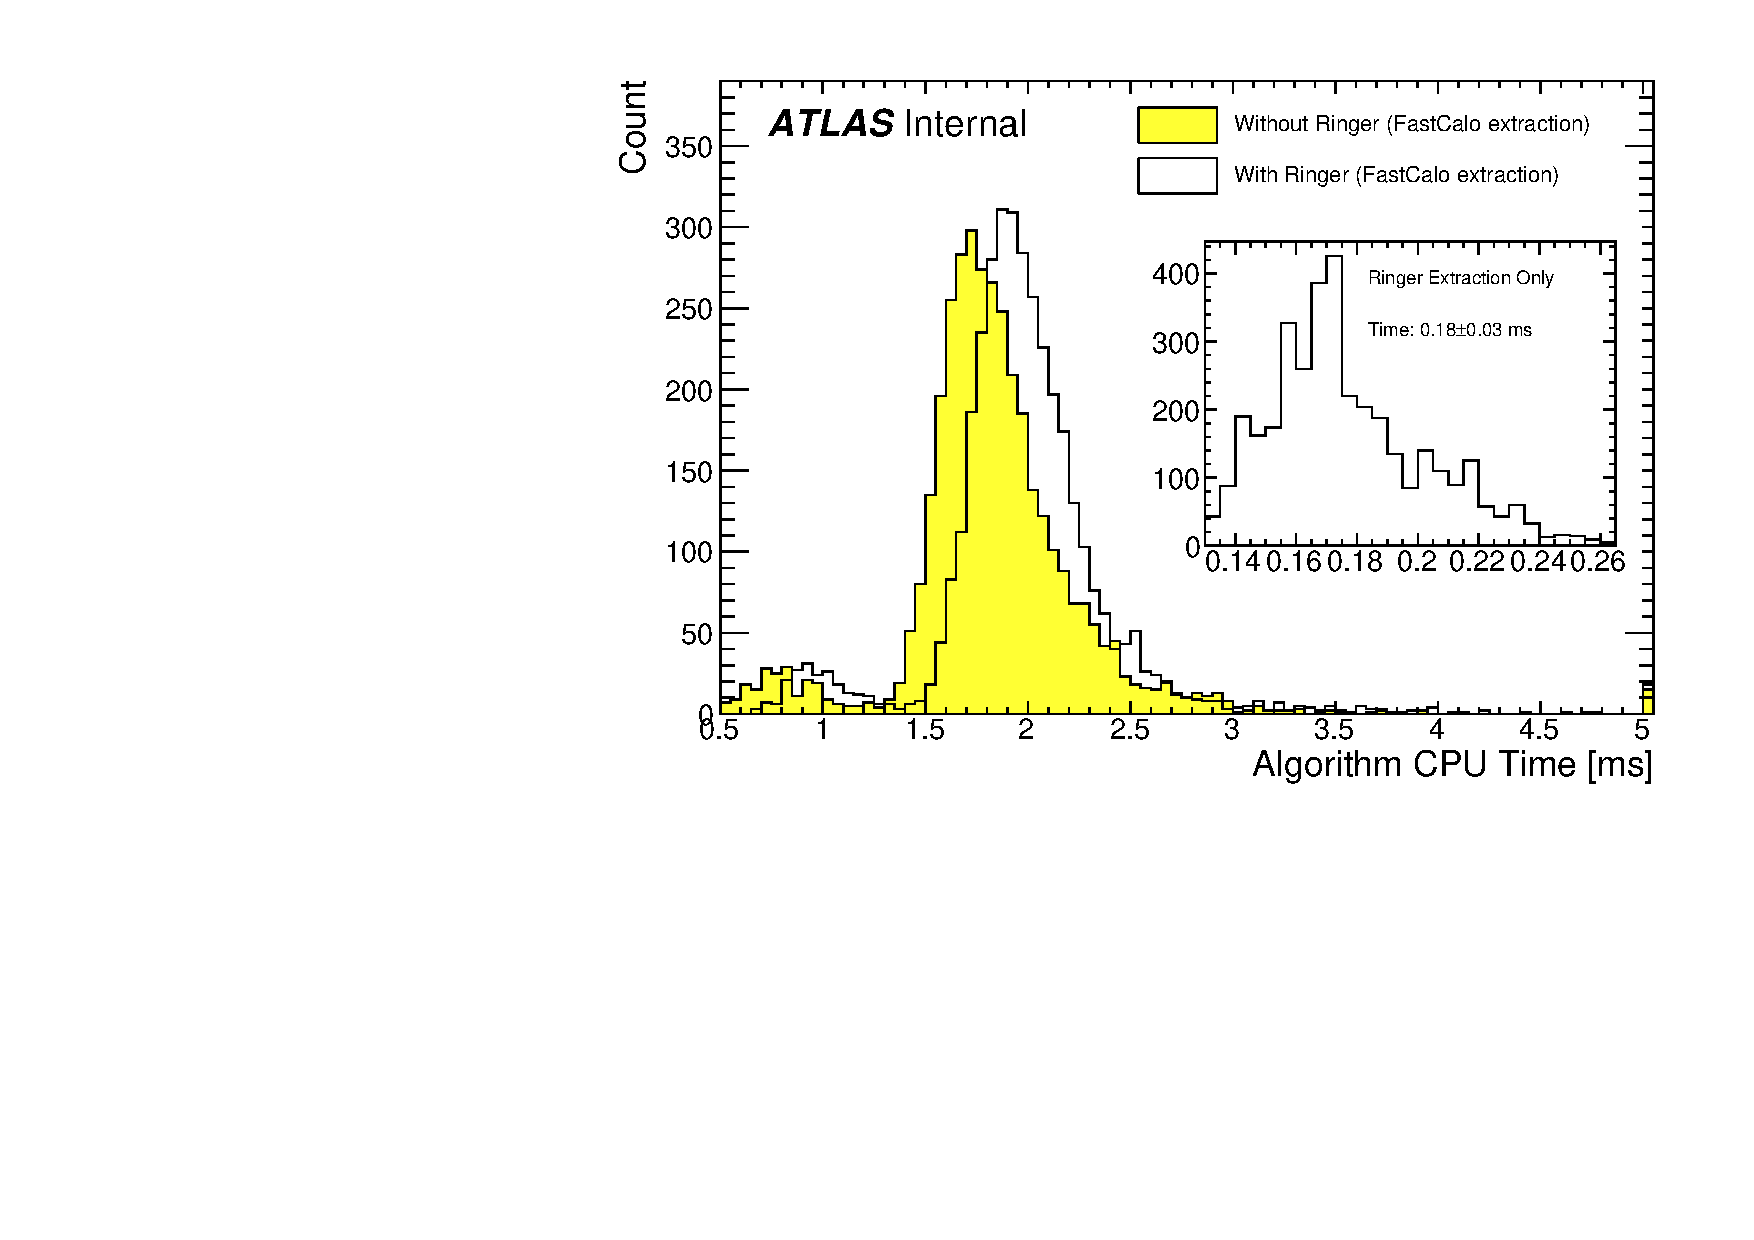
\includegraphics[width=.7\textwidth]{sections/operation/figures/EgammaFex_TotalTime}
	\centering
	\caption{\label{fig:fastcalo_fex_time}
		Total CPU time \textcolor{red}{per event} for the feature extraction algorithms in
		the \fastcalo step of electron triggers with (white) and without (yellow) \rnn{}
		using EB events ($\avgmu=45$ peak). Detail \textcolor{red}{on the right}
		shows the CPU time of the ring variable extraction. The CPU time does not
		include the (online) data preparation time.  Measurements were evaluated from 
		a very loose selection 
%		release AthenaP1-21.1.55 with a single electron trigger (e\_17\_lhvloose\_nod0)
		and with individual executions (independent measurements) in the same dedicated
		TDAQ node.
	}
\end{figure}

\begin{figure}[h!tb]
	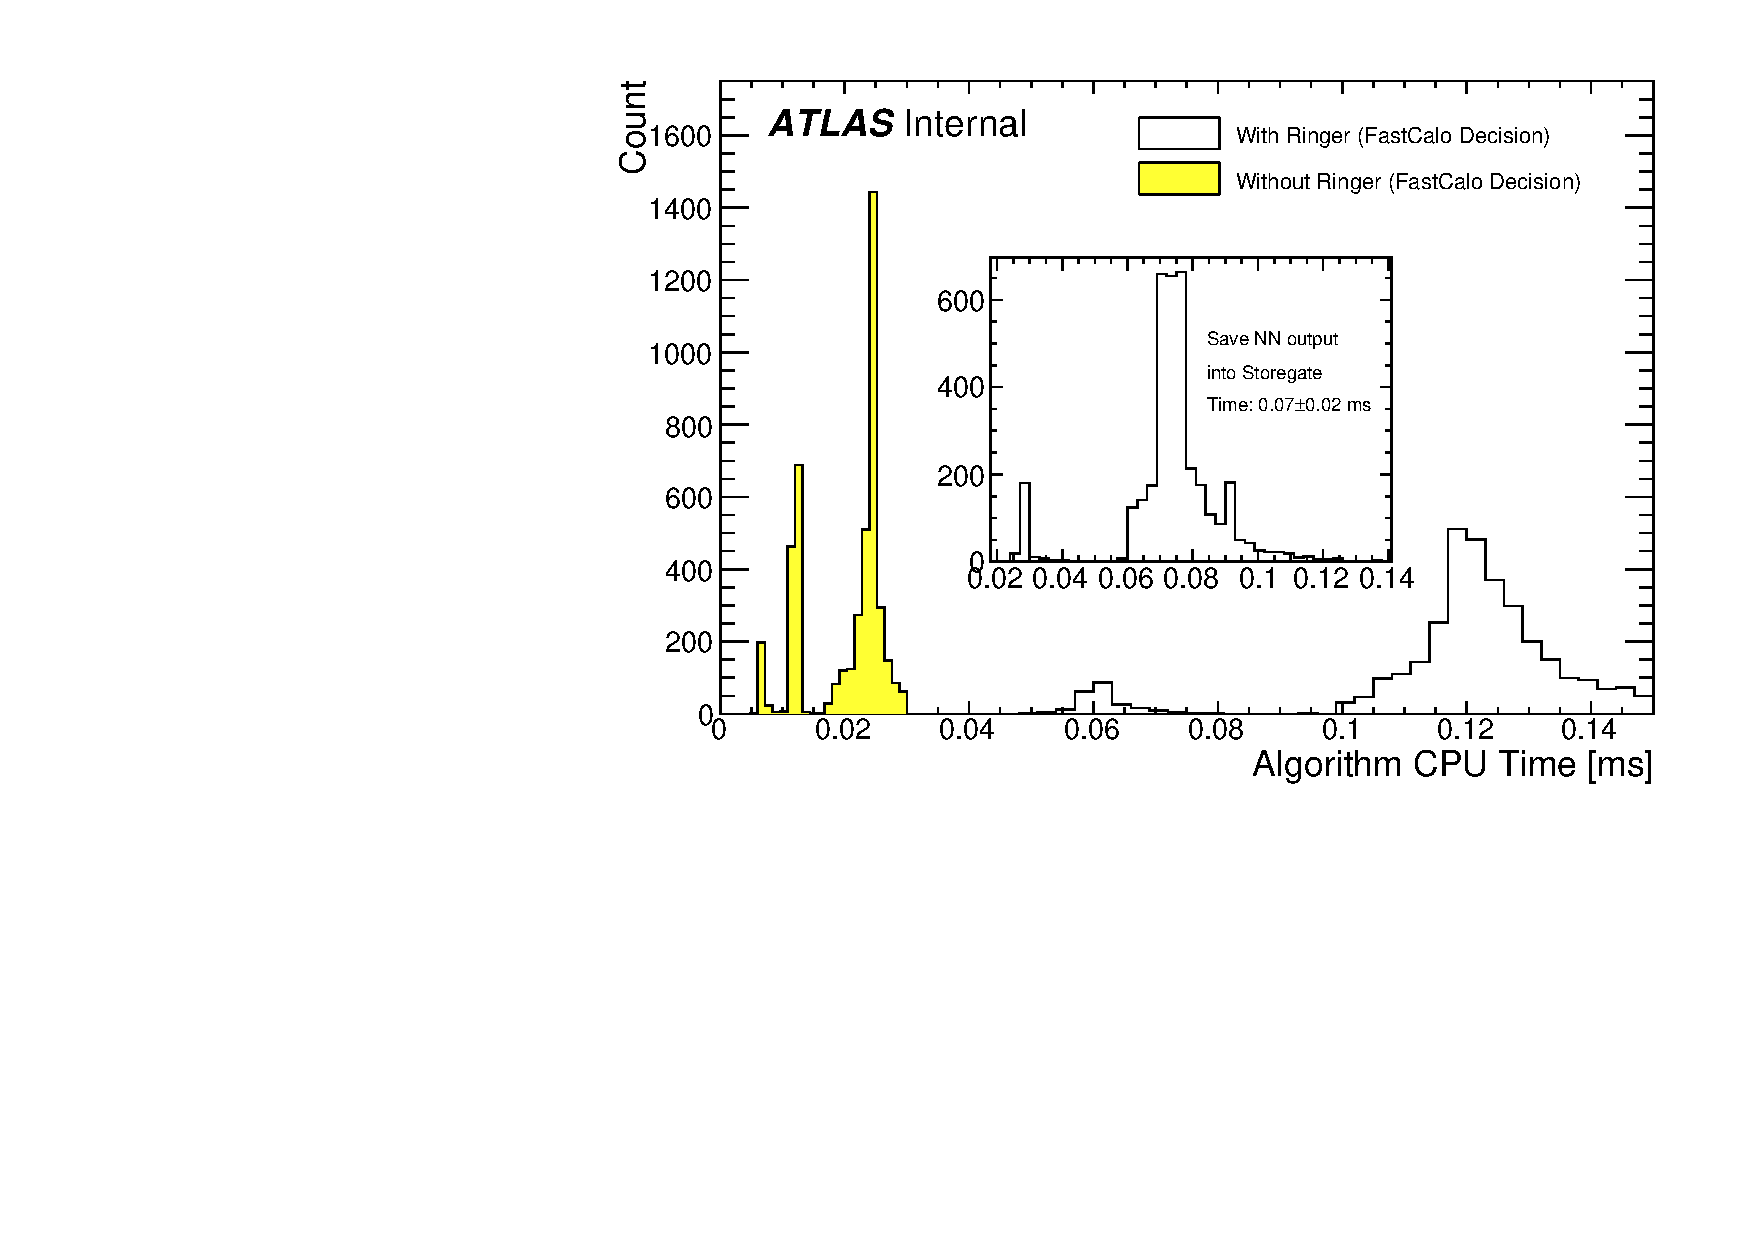
\includegraphics[width=.7\textwidth]{sections/operation/figures/EgammaHypo_TotalTime.pdf}
	\centering
	\caption{\label{fig:fastcalo_hypo_time}
		Total CPU time \textcolor{red}{per event} for the hypothesis testing algorithms
		in the \fastcalo step of electron triggers with (white) and without (yellow) \rnn{}
		using EB events. More details in description of Figure~\ref{fig:fastcalo_fex_time}. 
		The center histogram represents the CPU time to store the \rnn{} output into the AOD 
		format (persistence).}
\end{figure}

A multi-modal structure can be observed in the feature extraction distributions
of both trigger configurations, which is associated to the algorithm
for retrieving the EM2 cells and building related shower shape
variables\footnote{The three peak structure comes from the raw data conversion.
	Particularly, these are amongst the most-demanding contributions to
	the \fastcalo total CPU time.}. The computation of the ring variables, the only difference between the
triggers in the \fastcalo feature extraction, requires \textcolor{red}{an} additional \textcolor{red}{average} CPU time per
event of \SI{0.18 \pm 0.03}{\ms/\text{event}}. 
A less relevant contribution
comes from hypothesis testing, in which the ring variables are normalized, the
discriminant is computed, compared to the selection requirement and stored into
the AOD\footnote{For Run-3 this step has been removed as a way to reduce the CPU time at \fastcalo step.} 
persistent format. 
Specifically, \rnn{} hypothesis testing is considerably more demanding
(up to \SI{0.14}{\ms/\text{event}}), mostly due to the time 
to store the neural network output \SI{0.07 \pm 0.02}{\ms/\text{event}}, 
than the cut-based selection
(\SI{0.02}{\ms/\text{event}}), however small with respect to the feature
extraction values. 


Taking into account the referred values, the \rnn{} can require a
relative increase of up to \SI{50}{\%} in the \fastcalo{} CPU time per event
with respect to the trigger without \rnn{}\footnote{We expect the result to be
	dependent on the trigger configuration due to presence of pile-up. Reported
	results are for e17\_lhvloose\_nod0.}. Nonetheless, the \rnn{} contributes to
a more discriminant selection, \textcolor{red}{allowing to reduce CPU} demanding triggers
by reducing the processing of fake electron in the computationally demanding
subsequent steps as will be shown in the following subsection.

\FloatBarrier
\subsection{Estimated CPU Impact \textcolor{red}{on} the Lowest-Energy Threshold Unprescaled
	Single Electron Trigger}\label{top:cpu_e26}

\textcolor{red}{The} potential of saving CPU requirements by
avoiding the computation of fake candidates with the \rnn algorithms was demonstrated using} algorithms using the
lowest-energy-threshold unprescaled single electron trigger
\textcolor{red}{(tight criterion). This trigger algorithm was executed with}
%(tight criterion). We executed it with 
and without the \rnn{} algorithm in the same database using a dedicated node for processing.
In this measurement, we considered about 3,400 events from EB stream of run
327265 \textcolor{red}{processed with} release AthenaP1,21.1.55. The \rnn{} algorithm \textcolor{red}{provided an overall} 
\SI{60}{\%} reduction (\SI{30.72}{\milli\second} to \SI{10.36}{\milli\second})
in the CPU demands.


\section{Quadrant Analysis}\label{ssec:quadrant}

\textcolor{red}{In this approach, only data collected by the primary triggers whose selection is from its offline equivalent is considered\footnote{I.e., if a \tight{} trigger leg is being evaluated, we also apply \tight{} offline selection to the candidate.}.}
%In these analyses, we consider only data collected by the primary triggers and
%apply the trigger selection with its offline equivalent\footnote{I.e., if a
%\tight{} trigger leg is being evaluated, we also apply \tight{} offline
%selection to the candidate.}. 
Results in Section~\ref{top:quadrant_results} show
\textcolor{red}{trigger selection performance using} \tight{} requirement for the duplicated triggers during
2017.
%Thus, it allows to assess the direct impact of applying the \rnn{} selection
%with respect to the cut-based one, when keeping the tag selection fixed.

\subsection{Results}\label{top:quadrant_results}

% \begin{comment}

% \begin{figure}[p]
%   \centering
% \begin{subfigure}[c]{.32\textwidth}
% \centering
% \includegraphics[width=\textwidth]{sections/analyses/figures/quadrant_plots/HLT_e28_lhtight_nod0_noringer_ivarloose_HLT_e28_lhtight_nod0_ivarloose_reta_et4_eta0.pdf}
% \caption{}%
% \end{subfigure}
% \hfill
% \begin{subfigure}[c]{.32\textwidth}
% \centering
% 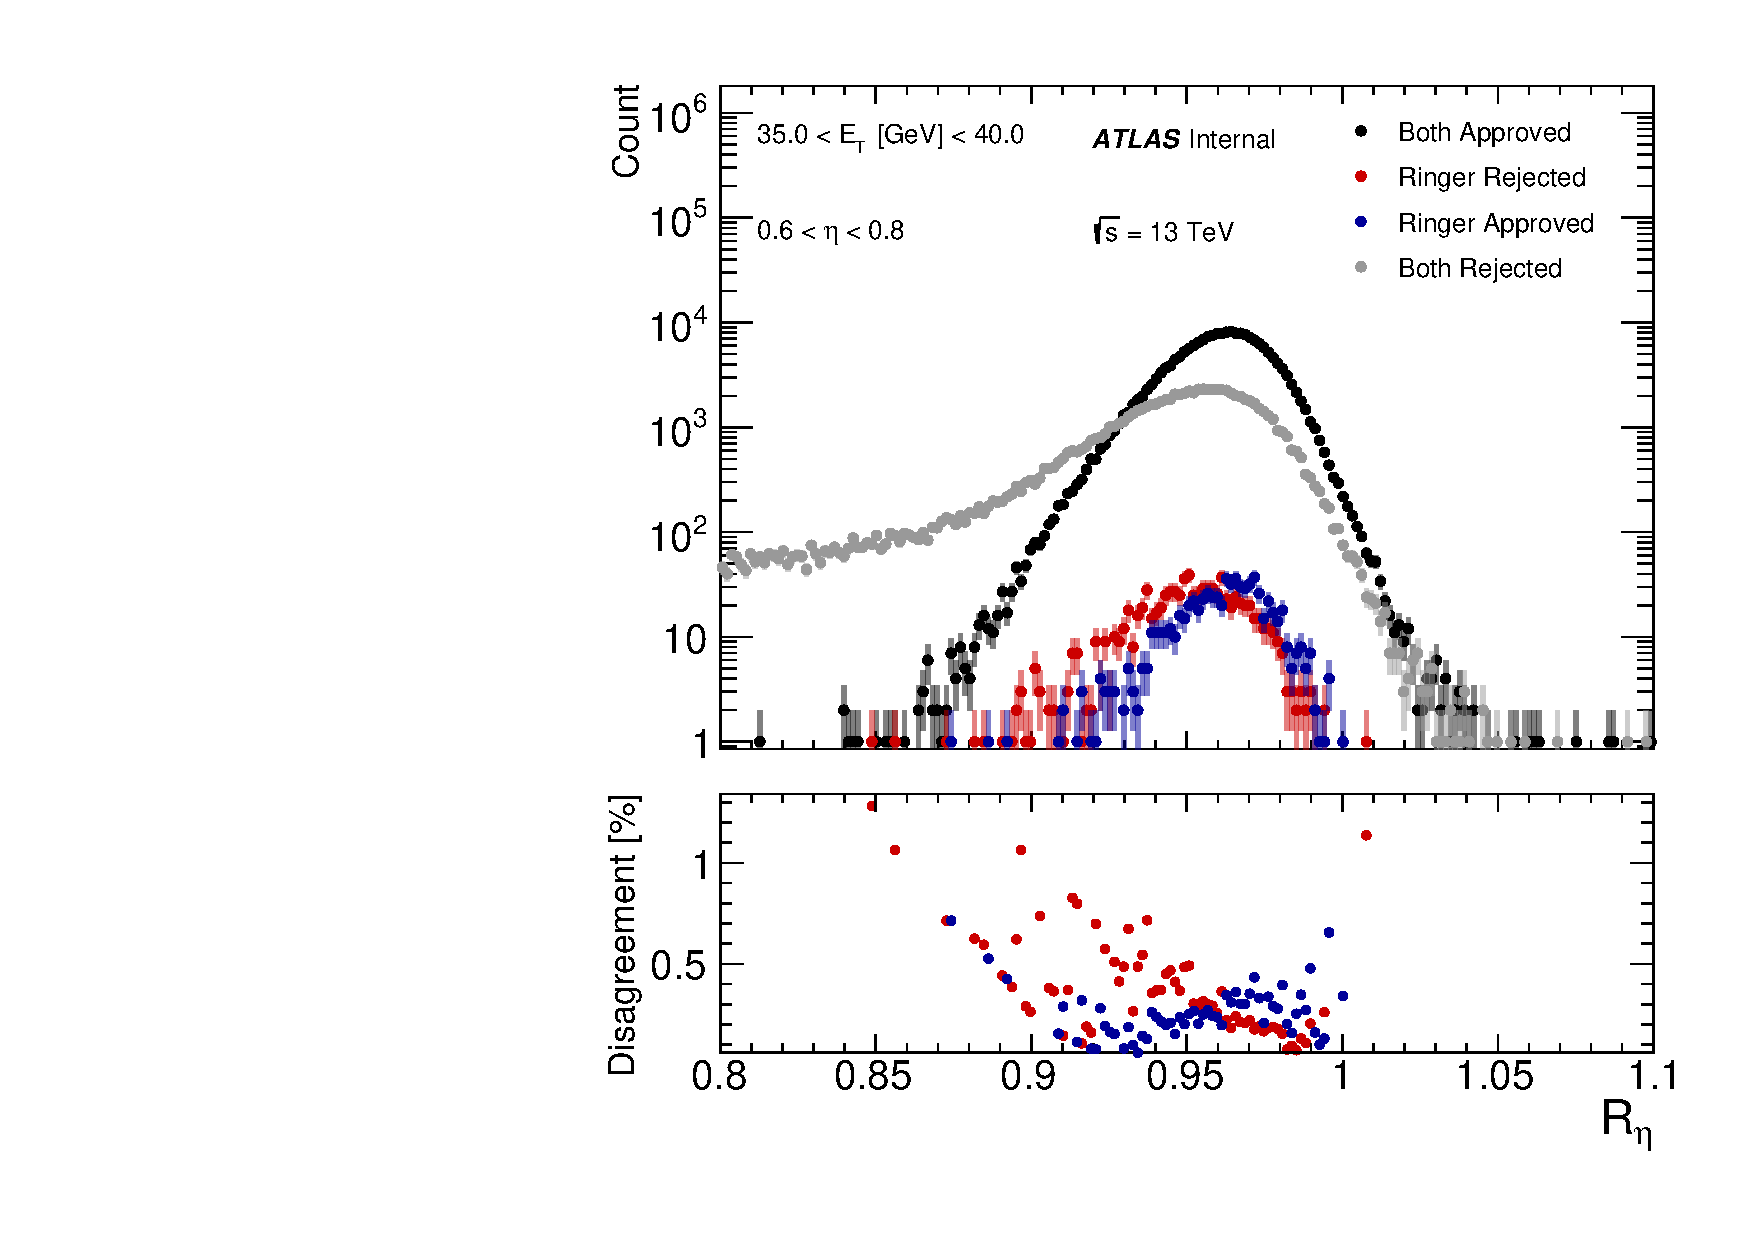
\includegraphics[width=\textwidth]{sections/analyses/figures/quadrant_plots/HLT_e28_lhtight_nod0_noringer_ivarloose_HLT_e28_lhtight_nod0_ivarloose_reta_et4_eta1.pdf}
% \caption{}%
% \label{fig:trigger_quadrant_reta1}
% \end{subfigure}
% \begin{subfigure}[c]{.32\textwidth}
% \centering
% \includegraphics[width=\textwidth]{sections/analyses/figures/quadrant_plots/HLT_e28_lhtight_nod0_noringer_ivarloose_HLT_e28_lhtight_nod0_ivarloose_reta_et4_eta2.pdf}
% \caption{}%
% \end{subfigure}
% \begin{subfigure}[c]{.32\textwidth}
% \centering
% \includegraphics[width=\textwidth]{sections/analyses/figures/quadrant_plots/HLT_e28_lhtight_nod0_noringer_ivarloose_HLT_e28_lhtight_nod0_ivarloose_reta_et4_eta3.pdf}
% \caption{}%
% \end{subfigure}
% \hfill
% \begin{subfigure}[c]{.32\textwidth}
% \centering
% \includegraphics[width=\textwidth]{sections/analyses/figures/quadrant_plots/HLT_e28_lhtight_nod0_noringer_ivarloose_HLT_e28_lhtight_nod0_ivarloose_reta_et4_eta4.pdf}
% \caption{}%
% \end{subfigure}
% \begin{subfigure}[c]{.32\textwidth}
% \centering
% \includegraphics[width=\textwidth]{sections/analyses/figures/quadrant_plots/HLT_e28_lhtight_nod0_noringer_ivarloose_HLT_e28_lhtight_nod0_ivarloose_reta_et4_eta5.pdf}
% \caption{}%
% \end{subfigure}
% \begin{subfigure}[c]{.32\textwidth}
% \centering
% \includegraphics[width=\textwidth]{sections/analyses/figures/quadrant_plots/HLT_e28_lhtight_nod0_noringer_ivarloose_HLT_e28_lhtight_nod0_ivarloose_reta_et4_eta6.pdf}
% \caption{}%
% \end{subfigure}
% \hfill
% \begin{subfigure}[c]{.32\textwidth}
% \centering
% \includegraphics[width=\textwidth]{sections/analyses/figures/quadrant_plots/HLT_e28_lhtight_nod0_noringer_ivarloose_HLT_e28_lhtight_nod0_ivarloose_reta_et4_eta7.pdf}
% \caption{}%
% \end{subfigure}
% \begin{subfigure}[c]{.32\textwidth}
% \centering
% \includegraphics[width=\textwidth]{sections/analyses/figures/quadrant_plots/HLT_e28_lhtight_nod0_noringer_ivarloose_HLT_e28_lhtight_nod0_ivarloose_reta_et4_eta8.pdf}
% \caption{}%
% \end{subfigure}
% \caption{\label{fig:quadrant_reta_30GeV}Quadrant analyses plots for the
%   offline-reconstructed \reta using standard \abseta regions ((a)-(i)) employed
%   in efficiency measurements within the $30<\et{}~[\text{GeV}]<$ slice. The
%   top pad in each figure shows the raw number of observations for the four
%   mutually exclusive cases: both with and without \rnn{} triggered (black); triggered only
%   with \rnn{} (blue); triggered only without \rnn{} (red); neither one triggered
%   (grey). With the same color code, bottom pad contains the percentage of each
%   group with respect to the sum of them. The both and neither triggering cases
%   are displayed using the left y-axis, whereas the single triggering cases are
% shown using the right y-axis.}%
% \end{figure}
% \end{comment}

\textcolor{red}{To begin with, Quadrant Analysis was done with the \reta{} variable, one of the} 
%We begin the Quadrant Analysis with the \reta{} variable for being one of the
most electron-jet discriminating variables employed in the likelihood
algorithm~\cite{aaboud2019electron}. As shown in Figure~\ref{fig:quadrant_calo_variables_30GeV_eta}, the disagreement (obtained by summing the cases accepted only by a single trigger between both triggers) is small and bounded for most cases at 1\% level for the coverage of all calorimetry variables. 
This behavior is also observed for \et{} slices. 
\textcolor{red}{One should note that the working points of both triggers are not  exactly the same, although the \rnn{} aimed at keeping the same signal efficiency as being achieved by the cut-based strategy and was operating as desired.  Thus, much of the differences reflect this difficulty. In other words, }
%One should note that the integral of the single trigger cases is related to the limitation in the precision of setting the working point of both triggers to be exactly the same. In other words, 
the difference in height of the blue and red profiles in Figure~\ref{fig:quadrant_calo_variables_30GeV_eta} is mainly due to the small differences in efficiencies between the two triggers.
\textcolor{red}{From the operation, it was realized that such matching was better in the $0.6<\abseta{}<0.8$ region. Hence, comparison between profiles is simpler to be performed there.}
%Hence, comparison between profiles is simpler to be performed in the $0.6<\abseta{}<0.8$, which exhibits very similar performance.

For all variables 
\textcolor{red}{in this region, both triggers behave very similarly, even if some slight shifts can be observed in few profiles.}
%in this region, it is possible to observe that both triggers also behave very similarly, with very low disagreement and slight shifts in some profiles. 
This is \textcolor{red}{the case of} \reta{} and \rphi{}, where the \rnn{} trigger is consistently collecting slightly more events in signal region, i.e. respectively with slight tighter showers in $\eta{}$ and $\phi{}$ in the EM2. The \rnn{} trigger behavior shows even lower effect in the \rhad{}, where tighter tails are observed, resulting in less electrons with 10\% to 30\% energy in EM1, 1\% to 2\% in EM3 and more than 4 GeV hadronic leakage. \eratio{} also shows a slight bias towards collecting more events in the signal region with the \rnn{} trigger. Interestingly, some few events are accepted by the trigger with \rnn{}, when $0.5<\eratio{}<0.7$. We suspect it to be due electrons resulting in from premature showers with barycenter near the edge of two strips


% \begin{comment}

% We begin the Quadrant Analysis with the \reta{} variable for being one of the
% most electron-jet discriminating variables employed in the likelihood
% algorithm~\cite{aaboud2019electron}.  As shown in
% Figure~\ref{fig:quadrant_reta_30GeV}, the disagreement (obtained by summing the
% cases accepted only by a single trigger between both triggers) is small and
% bounded for most cases at \SI{1}{\%} level for the coverage of all calorimetry
% variables. This behavior is also observed for \et{} slices. One should note that
% the integral of the single trigger cases is related to the limitation in the
% precision of setting the working point of both triggers to be exactly the same.
% In other words, the difference in height of the blue and red profiles in
% Figure~\ref{fig:quadrant_reta_30GeV} is mainly due to the small differences in
% efficiencies between the two triggers. Hence, comparison between profiles is simpler to be performed in the $0.6<\abseta{}<0.8$ slice
% (Figure~\ref{fig:trigger_quadrant_reta1}), which exhibits very
% similar.

% We dedicate to evaluate the profiles for the remaining calorimetry variables in
% this region, as shown in Figure~\ref{fig:quadrant_calo_variables_30GeV}. Again,
% it is possible to observe that both triggers behave very similarly, with very
% low disagreement and slight shifts in some profiles. This is the case of
% \reta{}, \rphi{} and \wstot{} where the \rnn{} trigger is consistently
% collecting slightly more events in signal region, i.e.\@ respectively with slight
% tighter showers in \eta{} and \phi{} in the \emii{}, and lower shower width in
% \emi{}. The \rnn{} trigger behavior shows even lower effect in the \rhad{},
% \fI{} and \fIII{}, where tighter tails are observed, resulting in less electrons
% with \SI{10}{\%} to \SI{30}{\%} energy in \emi{}, \SI{1}{\%} to \SI{2}{\%} in
% \emiii{} and more than \SI{4}{\GeV} hadronic leakage. \eratio{} also shows a
% slight bias towards collecting more events in the signal region with the \rnn{}
% trigger. Interestingly, some few events are accepted by the trigger with \rnn{}
% when $0.5<\eratio{}<0.7$. We suspect it to be due electrons resulting in from
% premature showers with barycenter near the edge of two strips.
% \end{comment}


\begin{figure}[h!]
\centering
\begin{subfigure}[c]{.49\textwidth}
\centering
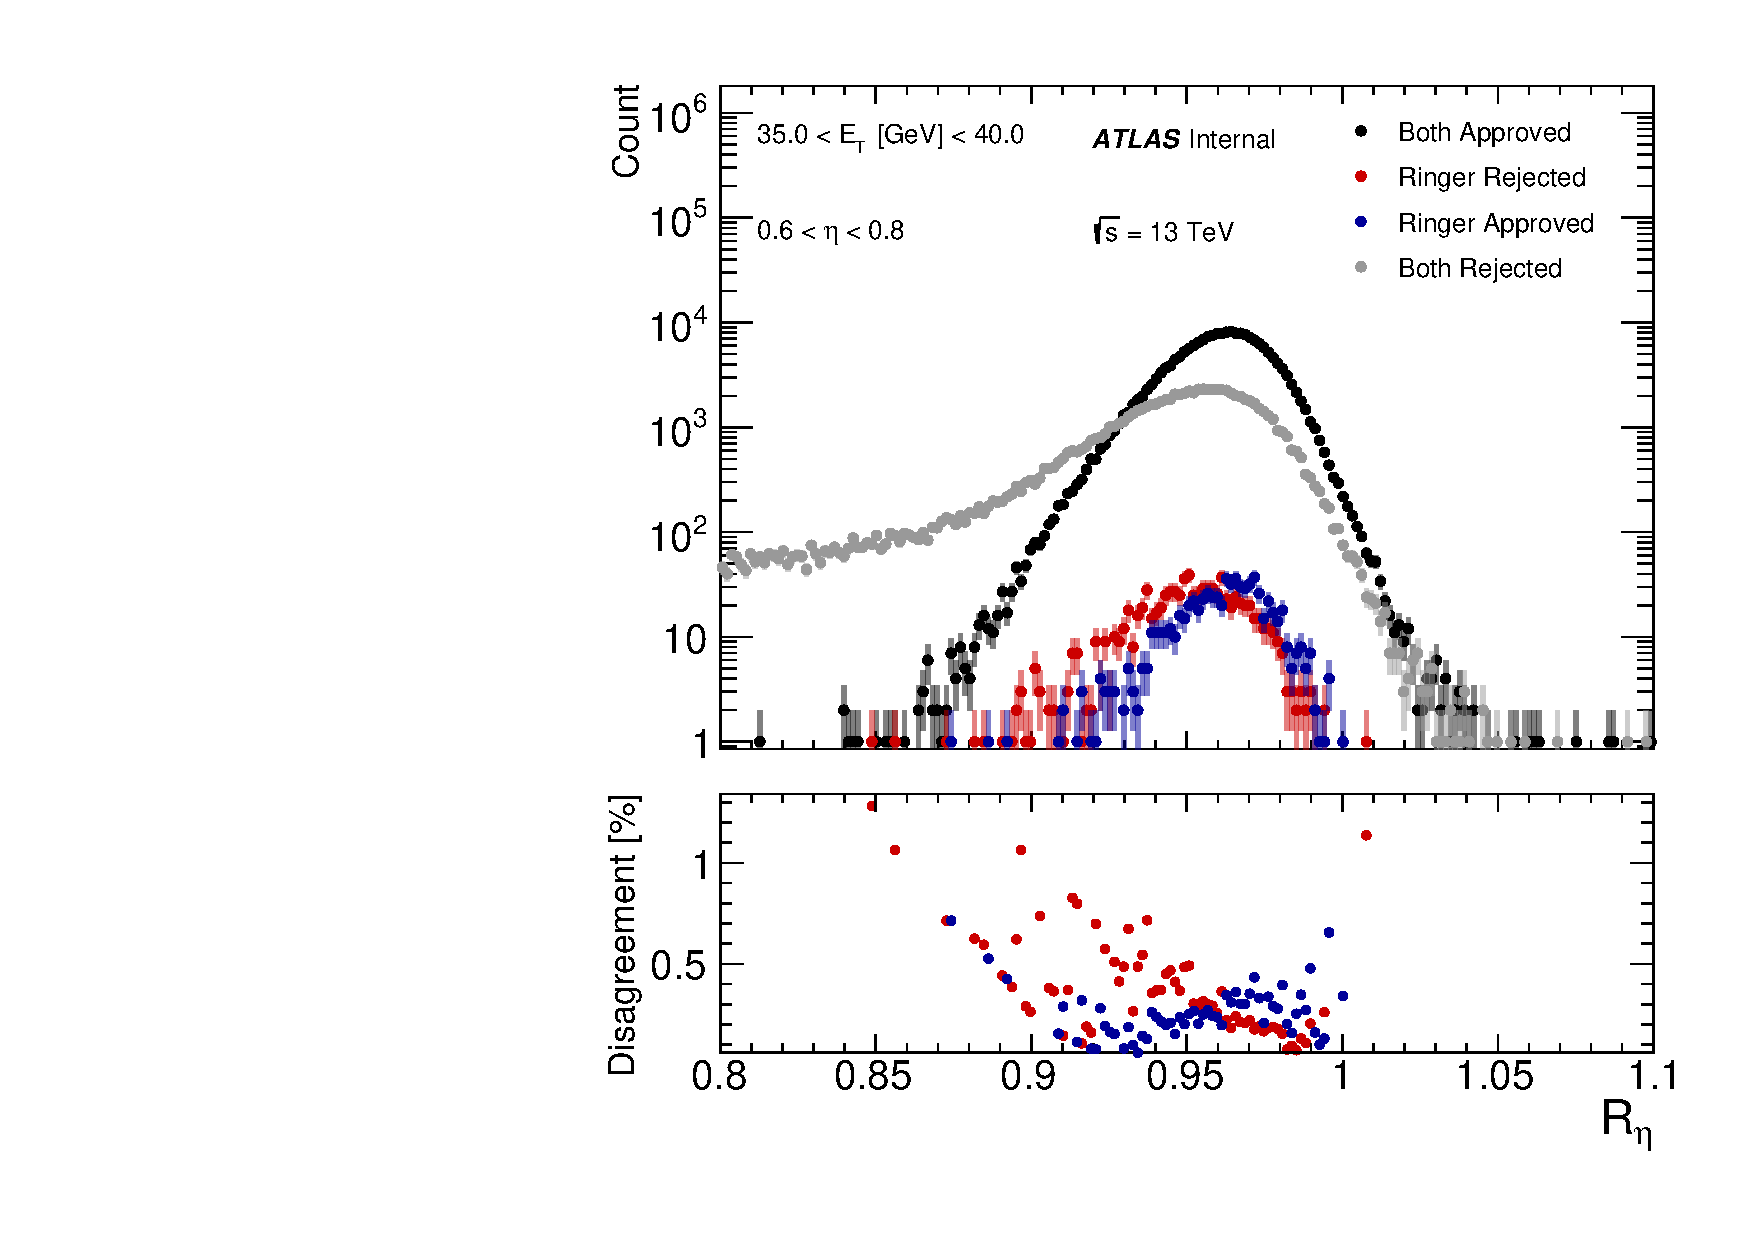
\includegraphics[width=\textwidth]{sections/analyses/figures/quadrant_plots/HLT_e28_lhtight_nod0_noringer_ivarloose_HLT_e28_lhtight_nod0_ivarloose_reta_et4_eta1.pdf}
\caption{}
\label{fig:quadrant_calo_variables_30GeV_eta}
\end{subfigure}
%\hfill
\begin{subfigure}[c]{.49\textwidth}
\centering
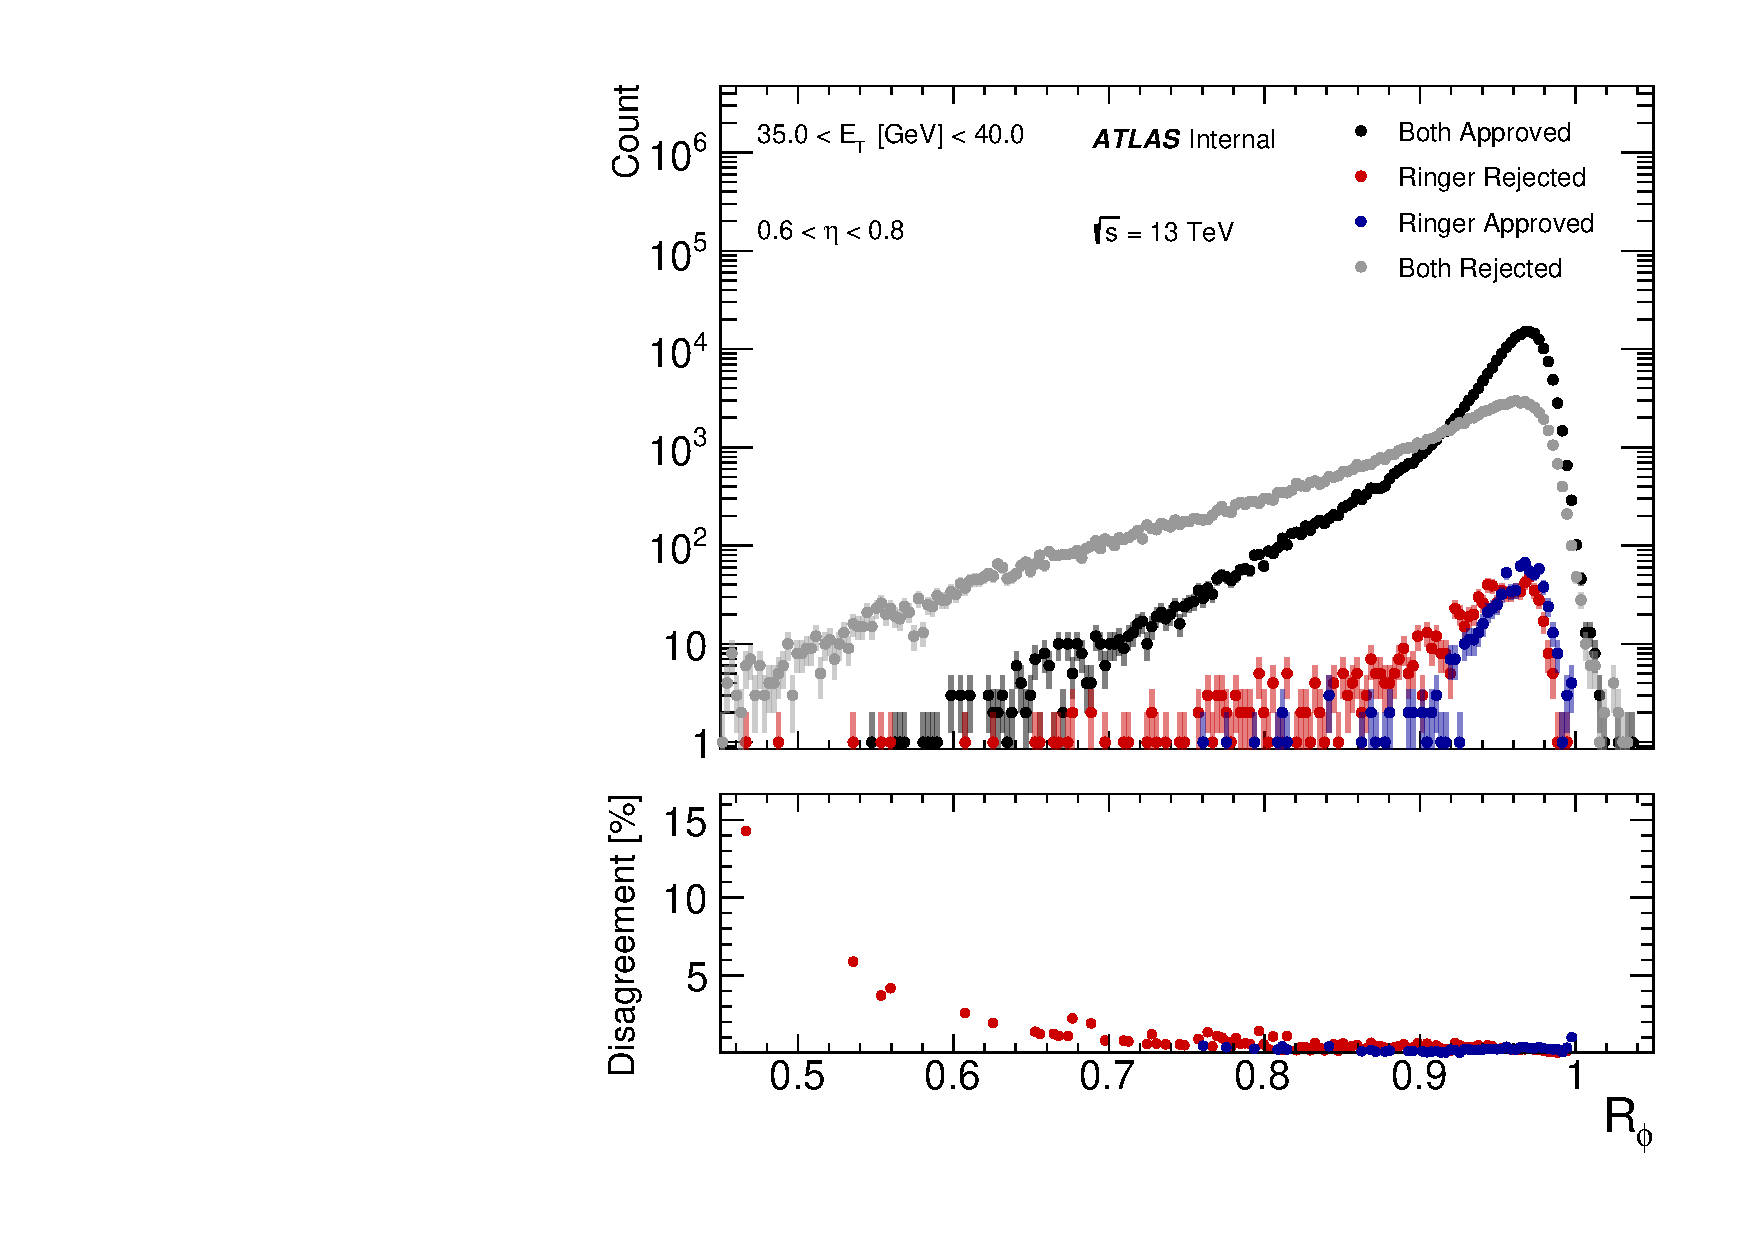
\includegraphics[width=\textwidth]{sections/analyses/figures/quadrant_plots/HLT_e28_lhtight_nod0_noringer_ivarloose_HLT_e28_lhtight_nod0_ivarloose_rphi_et4_eta1.pdf}
\caption{}
\end{subfigure} 
%\end{figure}
%\begin{figure}[p]\ContinuedFloat
\begin{subfigure}[c]{.49\textwidth}
\centering
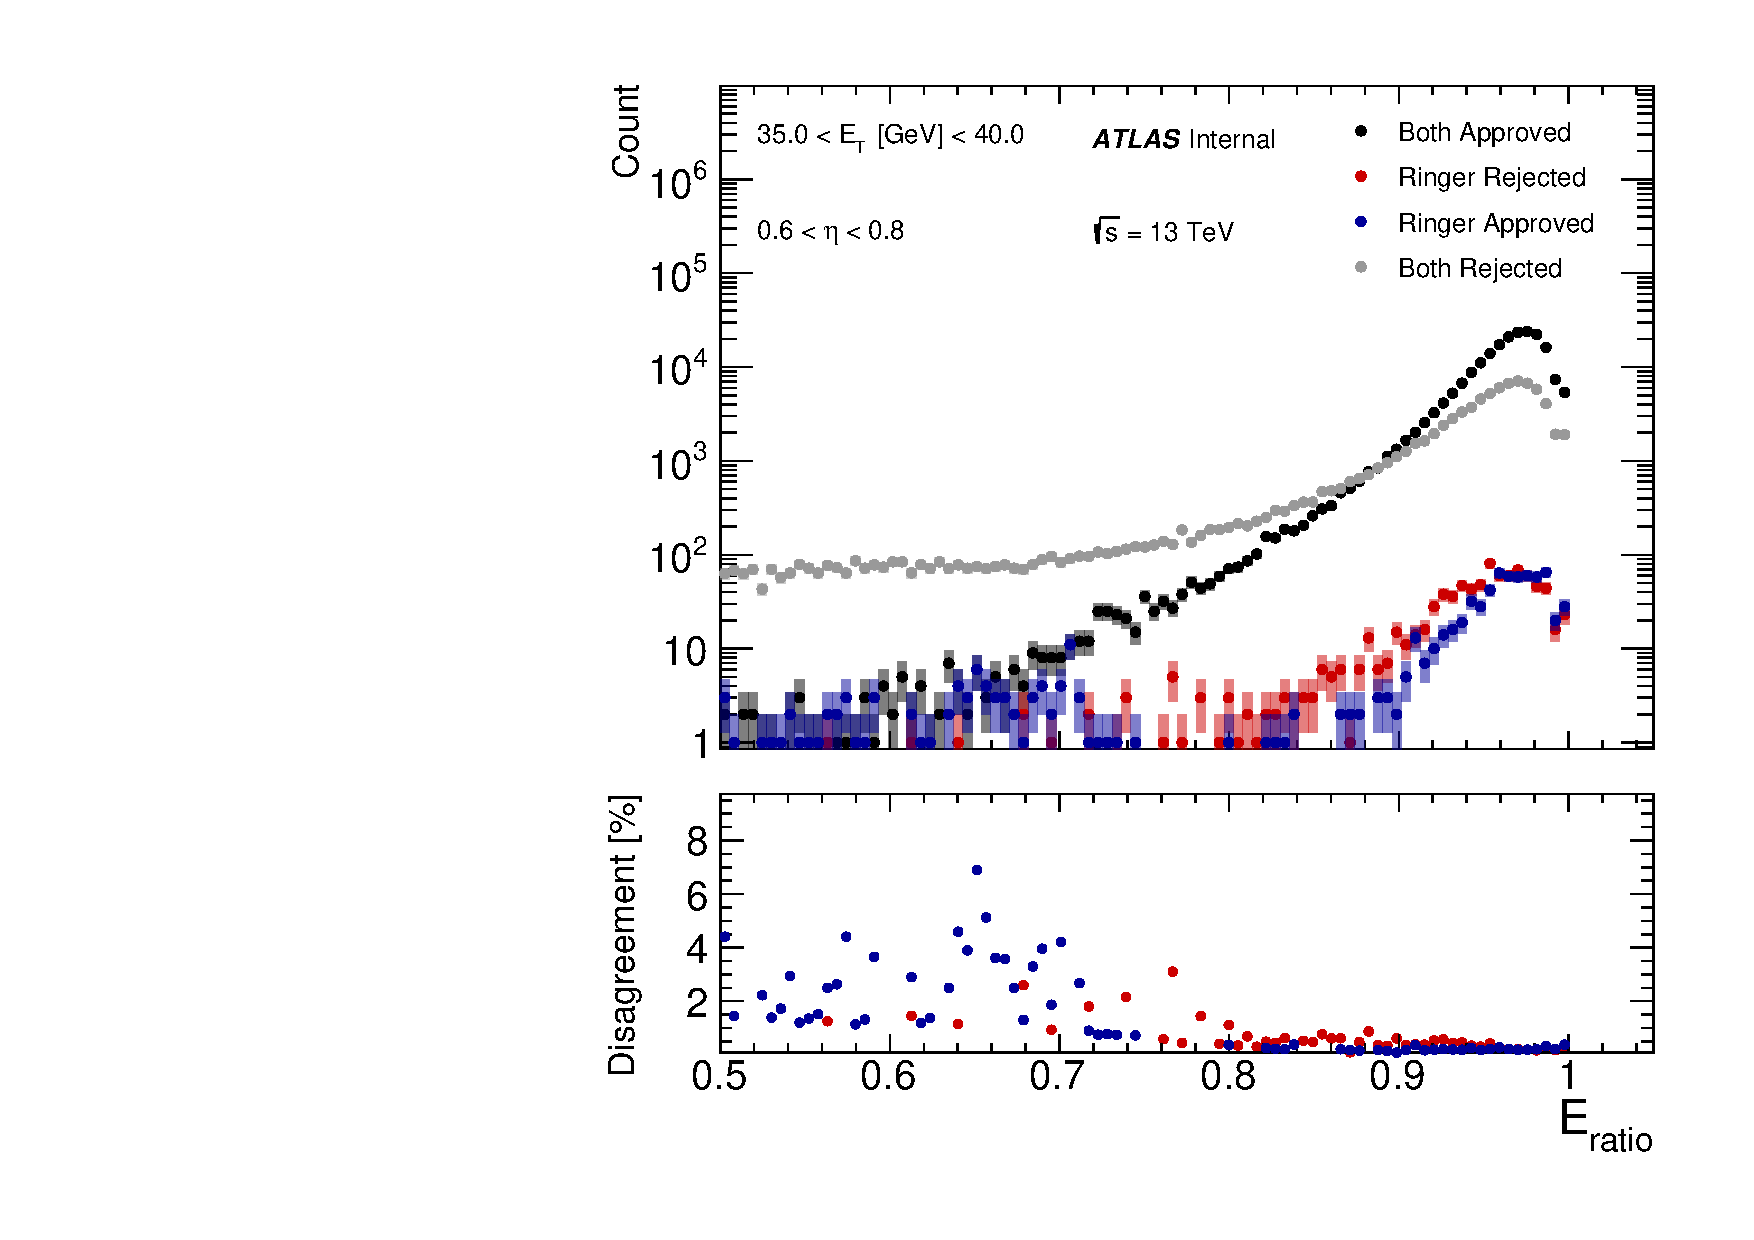
\includegraphics[width=\textwidth]{sections/analyses/figures/quadrant_plots/HLT_e28_lhtight_nod0_noringer_ivarloose_HLT_e28_lhtight_nod0_ivarloose_eratio_et4_eta1.pdf}
\caption{}
\end{subfigure}
\hfill
\begin{subfigure}[c]{.49\textwidth}
\centering
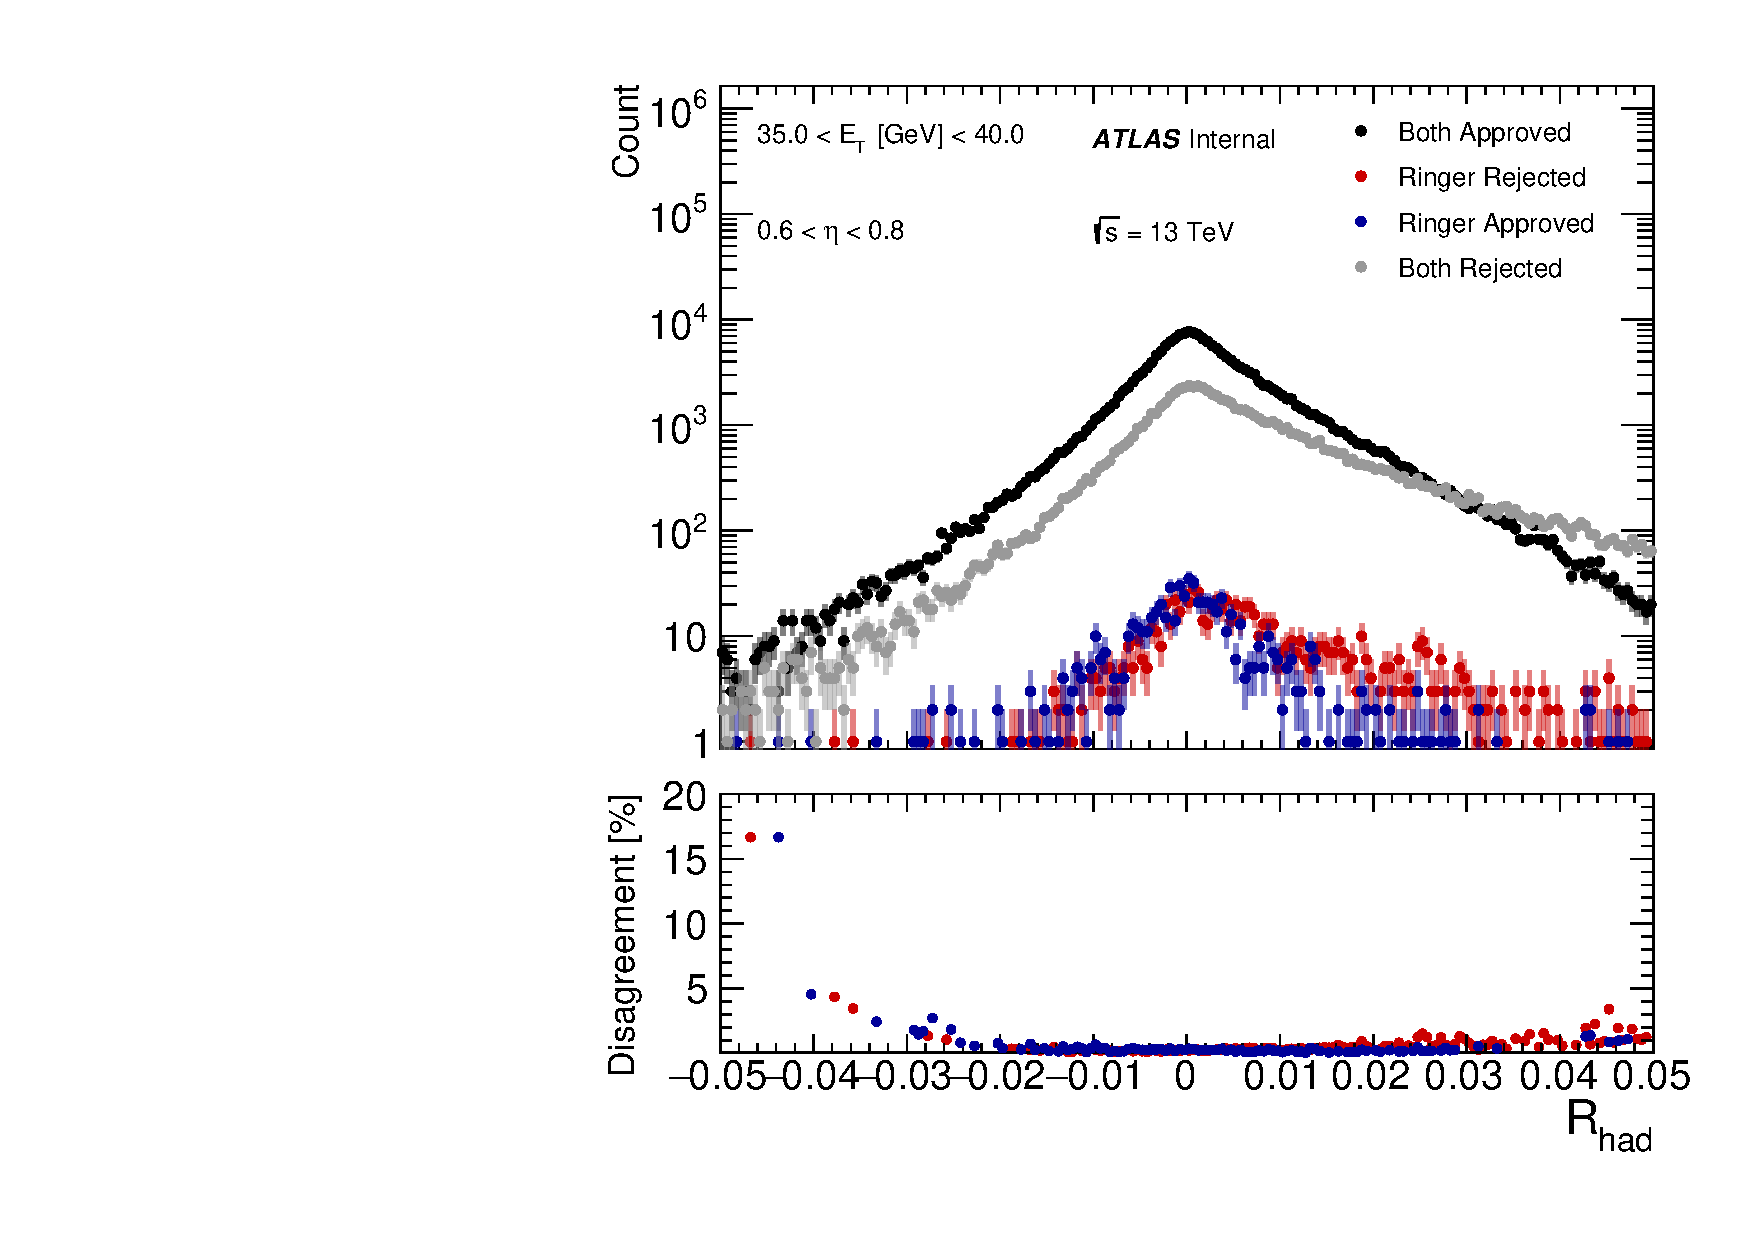
\includegraphics[width=\textwidth]{sections/analyses/figures/quadrant_plots/HLT_e28_lhtight_nod0_noringer_ivarloose_HLT_e28_lhtight_nod0_ivarloose_rhad_et4_eta1.pdf}
\caption{}
\end{subfigure} \\

% \begin{comment}

% \begin{subfigure}[c]{.49\textwidth}
% \centering
% \includegraphics[width=\textwidth]{sections/analyses/figures/quadrant_plots/HLT_e28_lhtight_nod0_noringer_ivarloose_HLT_e28_lhtight_nod0_ivarloose_weta2_et4_eta1.pdf}
% \caption{}%
% \label{fig:trigger_quadrant_weta2}
% \end{subfigure}
% \hfill
% \begin{subfigure}[c]{.49\textwidth}
% \centering
% \includegraphics[width=\textwidth]{sections/analyses/figures/quadrant_plots/HLT_e28_lhtight_nod0_noringer_ivarloose_HLT_e28_lhtight_nod0_ivarloose_wtots1_et4_eta1.pdf}
% \caption{}
% \end{subfigure} \\
% \end{figure}
% \begin{figure}[t]\ContinuedFloat
% \centering
% \begin{subfigure}[c]{.49\textwidth}
% \centering
% \includegraphics[width=\textwidth]{sections/analyses/figures/quadrant_plots/HLT_e28_lhtight_nod0_noringer_ivarloose_HLT_e28_lhtight_nod0_ivarloose_f1_et4_eta1.pdf}
% \caption{}

% \end{subfigure}
% \begin{subfigure}[c]{.49\textwidth}
% \centering
% \includegraphics[width=\textwidth]{sections/analyses/figures/quadrant_plots/HLT_e28_lhtight_nod0_noringer_ivarloose_HLT_e28_lhtight_nod0_ivarloose_f3_et4_eta1.pdf}
% \caption{}
% \end{subfigure}
% \end{comment}

\caption{%\label{fig:quadrant_calo_variables_30GeV}
	Quadrant analysis plots for the main offline-reconstructed
	calorimetry variables employed in the
	likelihood and for the $0.6<\abseta{}<0.8$ and
	$30<\et{}~[\text{GeV}]<35$ slices. 
	The top pad in each figure shows the raw number of observations for the four mutually exclusive cases: both with and without \rnn{}
	triggered (black); triggered only with \rnn{} (blue); triggered only without \rnn{} (red); neither one triggered (gray). With the same color code, \textcolor{red}{the bottom pad} contains the percentage of each group with \textcolor{red}{respect to the number of events selected by any trigger. The disagreement is defined by $(N_{blue}+N_{red})/(N_{blue}+N_{red}+N_{black}+N_{gray})$.}
}
%Quadrant analysis plots for the offline-reconstructed
%calorimetry variables employed in the
%likelihood and \wstot{} for the $0.6<\abseta{}<0.8$ and
%$30<\et{}~[\text{GeV}]<40$ slices.}%
\end{figure}

Although similar behavior is shown for the other 
\textcolor{red}{regions, the differences vary in strength in each \abseta{} region. As expected, }
%regions, the effects may present some variation in their strength according to each \abseta{} region. As expected, 
the trigger does not show a dependent behaviour with ID variables, as \textcolor{red}{shown} in Figure~\ref{fig:quadrant_track_variables_30GeV} for $35<\et{}~[\text{GeV}]<40$, since the only distinction between \textcolor{red}{them} is the electron identification model operating in the \fastcalo{}.

% \begin{comment}
% Although similar behavior is shown for the other regions, the effects may
% present some variation in their strength accordingly to each \abseta{} region,
% i.e.\@ larger or smaller shifts towards unitary \reta{} as shown in
% Figure~\ref{fig:quadrant_reta_30GeV}.
% Particularly, \weta{} and \fIII{} show changes in behavior
% depending on the \abseta{} regions, specially for bins $2.01<\abseta{}<2.37$ and
% $2.37<\abseta{}<2.47$. \weta{} profiles, depicted in
% Figure~\ref{fig:quadrant_weta_change_in_behavior}, seems to be nearly
% independent of the trigger employed when considering the $0.6<\abseta{}<0.8$
% region (Figure~\ref{fig:trigger_quadrant_weta2}), however regions
% $2.01<\abseta{}<2.37$ and $2.37<\abseta{}<2.47$ present a shift towards lower
% and larger shower widths, respectively. A similar behavior occurs for \fIII{},
% as shown in Figure~\ref{fig:quadrant_f3_change_in_behavior} the trigger with
% \rnn{} selection collects electrons with lower leakage in \emiii{} for region
% $2.01<\abseta{}<2.37$, whereas the opposite occurs in region
% $2.37<\abseta{}<2.37$. We believe this behavior to be associated with the usage of a single neural network during 2017 to cover the full end-cap region, but this could not be confirmed since 2018 data taking did not employ the duplicated trigger setup any longer.  As already mentioned, the $2.37<\abseta{}<2.37$ region is particularly different to the others due to the lack of the strips in EM1. Hence, the \rnn{} performance suffered deterioration at this region and, in order to keep the same signal efficiency, the operation point needed to be set looser, allowing the trigger to collect less signal-like electrons. This behavior is due to the usage of a single neural
% network during 2017 to cover the full end-cap region. As already mentioned, the
% $2.37<\abseta{}<2.47$ region is particularly different to the others due to the
% lack of the strips in \emi{}. Hence, \rnn{} performance suffered deterioration
% at this region and, in order to keep the same signal efficiency, the operation
% point needs to be set looser, allowing the trigger to collect less signal-like
% electrons.

% Figure~\ref{fig:quadrant_rhad_et4_eta4} shows a hump in the
% \rhad{} crack region. It occurs because the \itc{} cells are employed on the
% \rhad{} computation for all reconstruction frameworks (i.e. \fastcalo{}, \hlt{}
% and offline), despite energy contributions from electromagnetic showers can be
% captured by them. Particularly, the cut-based algorithm employs a $\rhadone{} <
% \SI{2.3}{\%}$ selection in this region\footnote{This threshold has a lower value
%   for the crack region than in the other ones. Despite resulting in a signal
% efficiency loss, the fake rate is still high in this region (see
% Figure~\ref{fig:e28_triggers} and Figure~\ref{fig:e28_triggers_fake} in
% Section~\ref{ssec:2017_ringer_operation}).}$^,$\footnote{It should be noticed
%   that the cut-based selection always employs \fastcalo{}-reconstructed
%   \rhadone{}, whereas the \rhad{} shown in the plots is equal to the
% offline-reconstructed \rhadone{} only if the electron lies within
% $0.8<\abseta{}<1.37$ (see Table~\ref{tab:IDcuts} in
% Section~\ref{ssec:std_variables}). Besides the differences in the reconstruction
% algorithms, the \rhad{} will usually have a larger hadronic leakage value than
% \rhadone{}, which explains the right tail with higher leakages than the cut in
% the \fastcalo ($\rhad>\SI{2.3}{\%}$) that is seen for the (black) profile where
% both \rnn{} and the cut-based triggers select the electrons in
% Figure~\ref{fig:quadrant_rhad_et4_eta4}.}, which is near the starting point of
% the second peak for the electrons accepted only by the \rnn{} selection, which
% points out that the neural network was able to keep a fraction of these electron
% showers deploying energy in the \itc{} cells.
% % FastCalo: https://acode-browser1.usatlas.bnl.gov/lxr/source/athena/Trigger/TrigAlgorithms/TrigT2CaloEgamma/src/EgammaHadEnFex.cxx?v=21.1
% % HLT, Offline: https://acode-browser1.usatlas.bnl.gov/lxr/source/athena/Reconstruction/egamma/egammaCaloTools/src/egammaIso.cxx?v=21.1#0054
% % T2Calo eta:   [0       0.6     0.8    1.15   1.37     1.52  1.81  2.01  2.37
% % T2Calo cuts:  [0.0588, 0.0564, 0.054, 0.048, 0.02376, 0.06, 0.06, 0.06, 0.054]
% % https://acode-browser1.usatlas.bnl.gov/lxr/source/athena/Trigger/TrigHypothesis/TrigEgammaHypo/src/TrigL2CaloHypo.cxx?v=21.1#0260

% As expected, the triggers do not show a dependent behavior with ID variables
% (Figure~\ref{fig:quadrant_track_variables_30GeV}) since the only distinction
% between them is the electron identification model operating in the \fastcalo{}.
% %Considerations concerning the ID-calorimeter combined variables are available in
% %Appendix~\ref{ssec:quadrant_combined}.


% \begin{figure}[h!tb]
% \begin{subfigure}[c]{.49\textwidth}
% \centering
% \includegraphics[width=\textwidth]{sections/analyses/figures/quadrant_plots/HLT_e28_lhtight_nod0_noringer_ivarloose_HLT_e28_lhtight_nod0_ivarloose_weta2_et4_eta7.pdf}
% \caption{}
% \end{subfigure}
% \hfill
% \begin{subfigure}[c]{.49\textwidth}
% \centering
% \includegraphics[width=\textwidth]{sections/analyses/figures/quadrant_plots/HLT_e28_lhtight_nod0_noringer_ivarloose_HLT_e28_lhtight_nod0_ivarloose_weta2_et4_eta8.pdf}
% \caption{}
% \end{subfigure} \\
% \caption{\label{fig:quadrant_weta_change_in_behavior}
% Quadrant analyses plots for the offline-reconstructed with the particular
% profile behavior for the \weta{} variable in regions $2.01<\abseta{}<2.37$ (a) and
% $2.37<\abseta{}<2.47$ (b) in the $35<\et{} [\text{GeV}]<40$ slices.}%
% \end{figure}


% \begin{figure}[h!tb]
% \centering
% \begin{subfigure}[c]{.49\textwidth}
% \centering
% \includegraphics[width=\textwidth]{sections/analyses/figures/quadrant_plots/HLT_e28_lhtight_nod0_noringer_ivarloose_HLT_e28_lhtight_nod0_ivarloose_f3_et4_eta7.pdf}%
% \caption{}
% \end{subfigure}
% \begin{subfigure}[c]{.49\textwidth}
% \centering
% \includegraphics[width=\textwidth]{sections/analyses/figures/quadrant_plots/HLT_e28_lhtight_nod0_noringer_ivarloose_HLT_e28_lhtight_nod0_ivarloose_f3_et4_eta8.pdf}%
% \caption{}
% \end{subfigure}
% \caption{\label{fig:quadrant_f3_change_in_behavior}
% Quadrant analyses plots for the offline-reconstructed with the particular
% profile behavior for the \fIII{} variable in regions $2.01<\abseta{}<2.37$ (a)
% and $2.37<\abseta{}<2.47$ (b) in the $35<\et{} [\text{GeV}]<40$ slices.}%
% \end{figure}

% \begin{figure}[h!tb]
% \centering
% \includegraphics[width=.6\textwidth]{sections/analyses/figures/quadrant_plots/HLT_e28_lhtight_nod0_noringer_ivarloose_HLT_e28_lhtight_nod0_ivarloose_rhad_et4_eta4.pdf}%
% \caption{Quadrant analysis plots for the offline-reconstructed with the
% particular profile behavior for the \rhad{} variable in the crack region
% ($1.37<\abseta{}<1.52$).\label{fig:quadrant_rhad_et4_eta4}}%
% \end{figure}
% \end{comment}

\begin{figure}[h!tb]
%\centering
%\begin{subfigure}[c]{.49\textwidth}
\centering
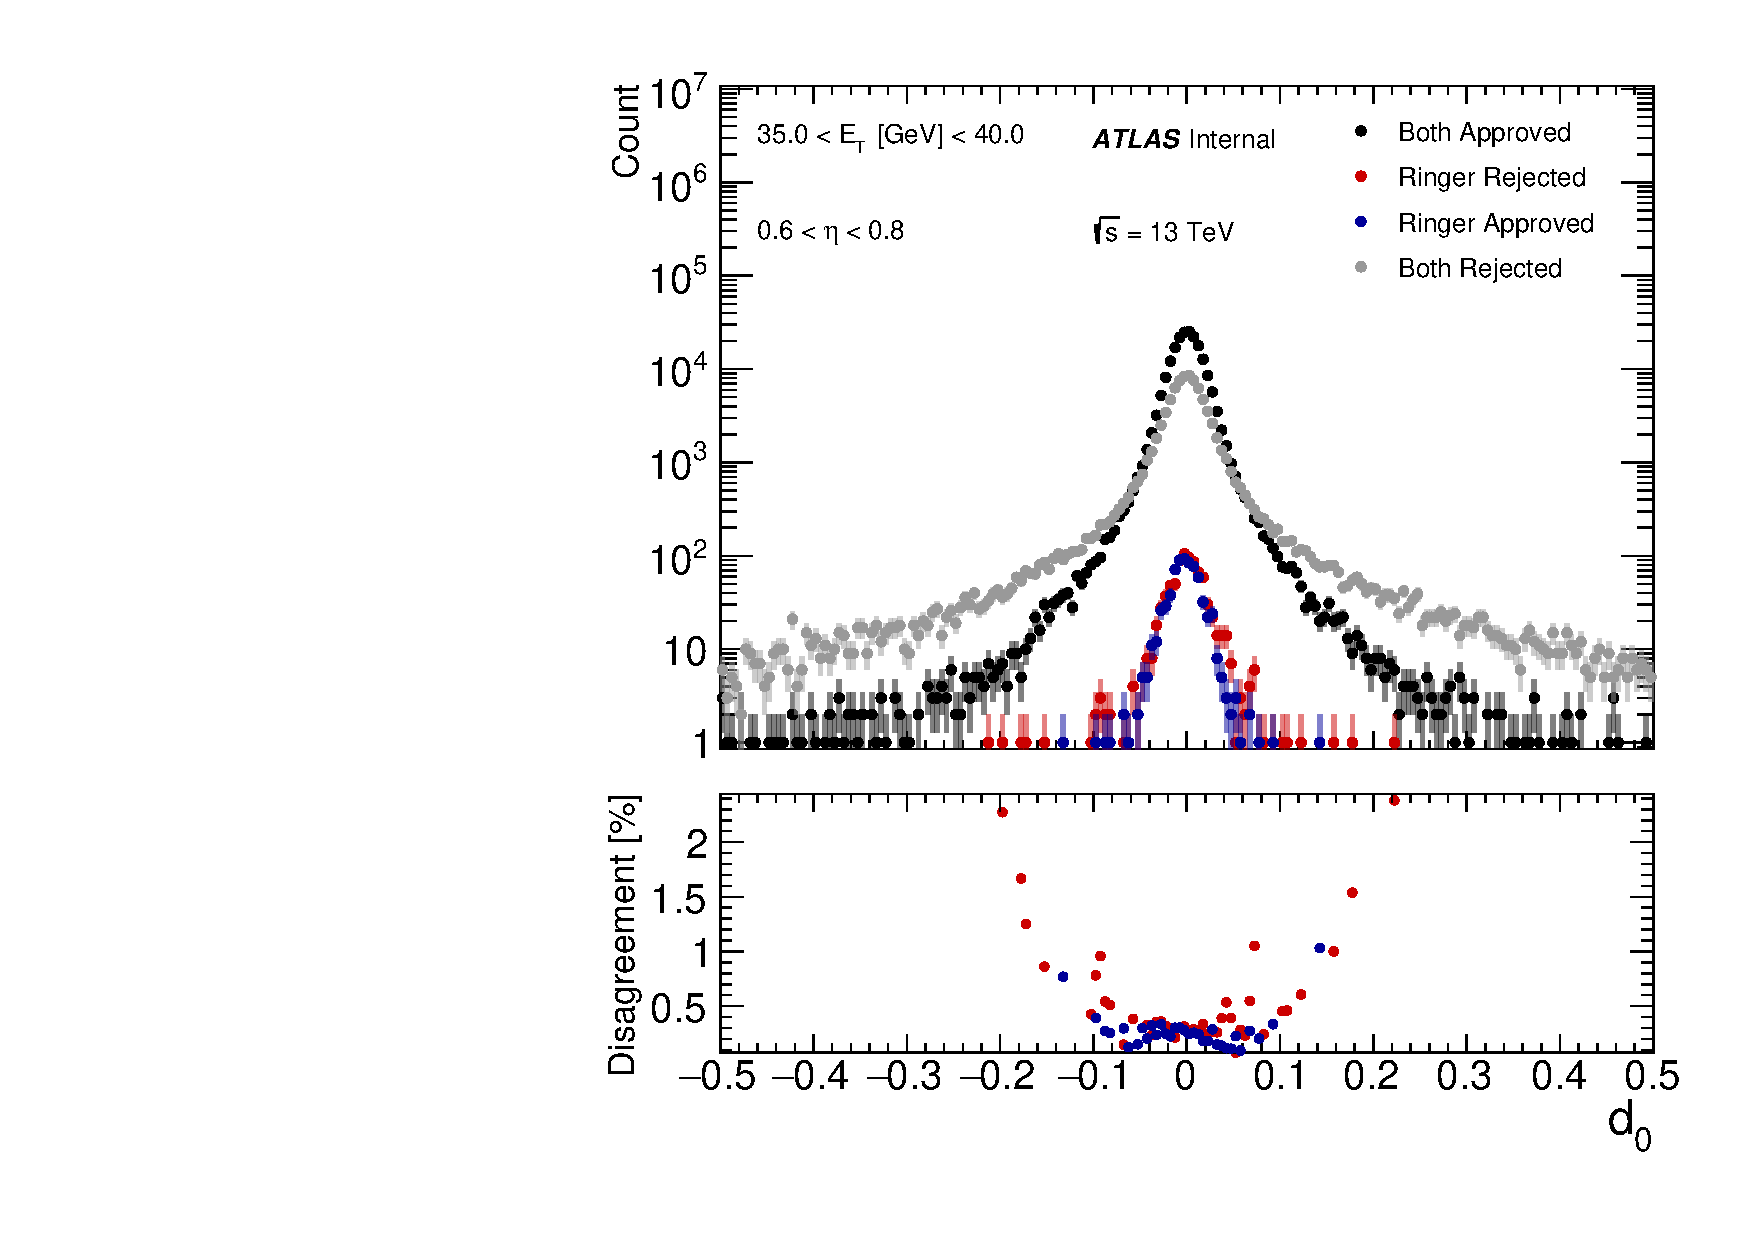
\includegraphics[width=.5\textwidth]{sections/analyses/figures/quadrant_plots/HLT_e28_lhtight_nod0_noringer_ivarloose_HLT_e28_lhtight_nod0_ivarloose_trackd0pvunbiased_et4_eta1.pdf}

%\end{subfigure}
%\hfill
%\begin{subfigure}[c]{.49\textwidth}
%\centering
%\includegraphics[width=\textwidth]{sections/analyses/figures/quadrant_plots/HLT_e28_lhtight_nod0_noringer_ivarloose_HLT_e28_lhtight_nod0_ivarlo%ose_d0significance_et4_eta1.pdf}
%\caption{}

%\end{subfigure} \\
%\begin{subfigure}[c]{.49\textwidth}
%\centering
%\includegraphics[width=\textwidth]{sections/analyses/figures/quadrant_plots/HLT_e28_lhtight_nod0_noringer_ivarloose_HLT_e28_lhtight_nod0_ivarloose_DeltaPOverP_et4_eta1.pdf}
%\caption{}

%\end{subfigure}
%\hfill
%\begin{subfigure}[c]{.49\textwidth}
%\centering
%\includegraphics[width=\textwidth]{sections/analyses/figures/quadrant_plots/HLT_e28_lhtight_nod0_noringer_ivarloose_HLT_e28_lhtight_nod0_ivarlo%ose_TRT_PID_et4_eta1.pdf}
%\caption{}

%\end{subfigure} \\
\caption{\label{fig:quadrant_track_variables_30GeV}
Quadrant analyses plots for the offline-reconstructed ID variable $d_0$ employed in the
likelihood for the $0.6<\abseta{}<0.8$ and $35<\et{}~[\text{GeV}]<40$ slice. \textcolor{red}{The $d_0$ variable is defined as Transverse parameter of the point of impact in relation to the collision beam.} 
}
\end{figure}

\FloatBarrier
\section[Agreement with respect to Previous
Trigger]{Agreement with respect to Previous Trigger}\label{ssec:agreement}

In this 
\textcolor{red}{analysis, the impact of using different triggers (from \rnn{} and cut-based algorithms) on the likelihood algorithm is evaluated. This }
%analysis, we observe how the usage of the different triggers (from \rnn{} and cut-based algorithms) may impact the likelihood algorithm. This 
study requires a pair of duplicated triggers (with and without the \rnn{}) operating online together. 
\textcolor{red}{The motivation for the choice of the duplicated trigger pairs has been discussed in Section~\ref{top:duplicated}. This analysis is performed using} 
%motivation for the choice of the duplicated trigger pairs in Section~\ref{top:duplicated}. Particularly, we perform this analysis using 
\Zee{} \tnp{} data, which were selected with the trigger requirement set to either one of the duplicated triggers for the tag, whereas the probe selection is invariably set to the offline \vloose{} criterion. This is the exact setup \textcolor{red}{employed by ATLAS to derive} the offline likelihood \textcolor{red}{for electrons above \SI{15}{\GeV}. To benefit} from the full 2017 statistics, data collected previous to the TS1 were also employed. In case the profiles are statistically identical, then it is expected that the \rnn{} trigger \textcolor{red}{does} not cause any relevant alteration in the derivation of the offline likelihood pdfs.  The statistical method for profile evaluation is described in Section~\ref{top:homogeneity_method} and the results are available in Section~\ref{top:agreement_homogeneity_results}.

%In this analysis, we dedicate to observe how the usage of different triggers may
%impact the likelihood algorithm. %Although a new trigger configuration
%aims at causing an improvement in the overall electron efficiency, one
%compelling property would be a nearly immutable trigger operation when seen by
%the offline selection algorithm regardless of the online configuration, given it
%reduces the effort in processing the full Run~2 data.
%This study requires a pair of duplicated triggers (with and without the \rnn{}) operating online together. We discuss the
%motivation for the choice of the duplicated trigger pair in
%Section~\ref{top:duplicated}. Particularly, we perform this analysis using
%\Zee{} \tnp{} data selected with the trigger requirement set to either one of
%the duplicated triggers for the tag, whereas the probe selection is invariably
%set to the offline \vloose{} criterion. It is the exact setup employed for
%deriving the offline likelihood for electrons above \SI{15}{\GeV}, except for
%the trigger selection used on the tags. To benefit from the full 2017
%statistics\footnote{Except for the special lumiblocks in the first three GRL
%runs resulting in a negligible luminosity loss of \SI{13}{\per\nano\barn}.},
%data collected previous to the TS1 are also employed. 
%In case the profiles are statistically identical, then it is expected that the
%\rnn{} trigger did not cause any relevant alteration in the derivation of the
%offline likelihood pdfs. The statistical method for evaluation of the profiles
%is described in Section~\ref{top:homogeneity_method} and the results are
%available in Section~\ref{top:agreement_homogeneity_results}.

\subsection{Duplicated Trigger Setup}\label{top:duplicated}

\textcolor{red}{Choosing a duplicated trigger configuration was made} 
%The choice of having a duplicated trigger was made 
taking into account the
monitoring purposes required \textcolor{red}{by} the efficiency evaluations shown in
Section~\ref{ssec:2017_ringer_operation} and to allow the agreement analysis described \textcolor{red}{here. To define the duplicated trigger, the following criteria were considered:}


\begin{enumerate}
  \item the lowest energy-threshold unprescaled single electron trigger employs the \tight requirement;%the lowest energy-threshold unprescaled single electron trigger employs
    %the \tight requirement, thus the employment of other criteria at similar
    %energy-threshold would imply in the usage of pre-scale factors\textcolor{red}{, due to the high events rate.};
  \item \textcolor{red}{the \tight requirement aims at selecting a high purity sample and, thus, may show better the disagreements between two triggers of distinct configuration. }Hence, any discrepancies would be seen already with low statistics for this requirement;%likewise, the \tight requirement operates at lower efficiency
    %and, thus, is subject to larger disagreement between two triggers of
    %distinct configuration. Hence, it is expected that the discrepancies appear
    %first (i.e. with lower statistics) for this requirement;
  \item in addition, as the \tight requirement aims at selecting a high purity electron sample, it limits the trigger decision 
  \textcolor{red}{boundary of the trained model, which was extracted with the same conditions and data for all operation requirements} 
  %boundary, extracted with the same conditions and data for all requirements, 
  to comprise a smaller signal region\footnote{Region where samples are labelled by the algorithm as electrons.} for both triggers\footnote{It is worth mentioning that the \rnn{} and cut-based algorithms were optimized on different datasets, but the requirement definitions were kept fixed for the same conditions for each algorithm except for the targeted efficiencies.}, therefore resulting in larger divergences between the algorithms;
  
%in addition, the \tight requirement limits the decision boundary,
%    extracted with the same conditions and data for all requirements, to
%    comprise a smaller signal region\footnote{Region where samples are labelled by the algorithm
%    as electrons.} for both triggers\footnote{It is worth mentioning that the
%     \rnn{} and cut-based algorithms were optimized on different datasets, but
%      the requirement definitions were kept fixed for the same conditions for
%    each algorithm except for the targeted efficiencies.}, therefore resulting
%    in larger divergences between the algorithms;
  \item a lower CPU reduction results \textcolor{red}{when} more triggers are duplicated;
  \item although higher energy-thresholds result in lower CPU demands, the
    primary single electron triggers are not very computationally demanding;
  \item it is preferable to keep a duplicated trigger with energy-threshold as
    near as possible to the lowest unprescaled one, since less changes in the
    systematic parameters employed in the \Zee{} \tnp{} method take place;
  \item given that the \rnn{} was employing new variables and a neural network
    strategy for the first time, it was considered to prioritize obtaining as
    much data as possible to allow the characterization of possible subtle
    changes caused by the new trigger;
  \item since it was unclear how much statistics would be required \textcolor{red}{observe possible} differences in the behaviors, we decided to constrain the
    duplicated trigger to operate without pre-scale.
\end{enumerate}

As a result, it was decided to \textcolor{red}{duplicate only a single} electron trigger with energy-threshold as near as possible from the primary trigger and to keep it unprescaled.

%As a result, it was decided to duplicate a solely single electron trigger with
%energy-threshold as near as possible from the primary trigger and to keep it
%unprescaled. Namely, the e28\_lhtight\_nod0\_noringer\_ivarloose trigger with
%the cut-based algorithm is the duplicated setup for the
%e28\_lhtight\_nod0\_ivarloose trigger, which operated with \rnn{} algorithm in
%the \fastcalo{} step.

\subsection{Method}\label{top:homogeneity_method}



We approach the problem based on homogeneity tests on histograms~\cite{homogeneity_test}\footnote{It is based on a test originally developed by Pearson~\cite{pearson1911probability} and popularly employed in many fields beyond HEP, e.g. social sciences~\cite{wickens2014multiway} and health~\cite{ma2015homogeneity}, usually labelled as contingency or consistency tests.}, in order to \textcolor{red}{check for (systematic) effects of} the trigger configuration.
%We approach the problem based on homogeneity
%tests~\cite{homogeneity_test}\footnote{It is based on a test originally
%  developed by Pearson~\cite{pearson1911probability} and popularly employed in
%  many fields beyond HEP, e.g. social sciences~\cite{wickens2014multiway} and
%health~\cite{ma2015homogeneity}, usually labelled as contingency or consistency
%tests.} to check how relevant, if existent, is the (systematic) effect of the
%trigger configuration in the profiles with respect to statistical effects.

In order to benefit from the test without having to customize it to the particular analysis setup, we proceed the following way. First, we split data into two
statistically independent groups attempting to keep data taking conditions as
similar as possible by successively taking data to each group from small
consecutive periods. Ideally, it would be desired to split data using luminosity
blocks for achieving nearly the same conditions. However, technical limitations
constrained the period to larger time scales, hence allowing the test to
indicate that the two groups are originating from different populations due to
confounding variables. 
Either way, it does not affect the goal of this assessment. By comparing the p-values of the two groups, we can evaluate how the different configuration affects the likelihood of the profiles to be drawn from the same distribution. If the p-values\footnote{\textcolor{red}{The p-value here is defined by: $P-value \approx f(x, k) = \frac{1}{2^{k/2}\Gamma(k/2)}x^{k/2 -1}e^{-x/2}$}} have negligible fluctuations with respect to the values obtained by the tests comparing the same triggers, then the systematic effect in the profiles is negligible with respect to half\footnote{Once each group is using nearly half of the integrated luminosity.} of the statistics available
%Either way, it does not affect the goal of this assessment. 
%By comparing the p-values of the two groups, we can evaluate how the
%different configuration affects the likelihood of the profiles to be drawn from
%the same distribution. If the p-values have negligible fluctuations with respect
%to the values obtained by the tests comparing the same triggers, then the
%systematic effect in the profiles is negligible with respect to
%half\footnote{Once each group is using nearly half of the integrated
%luminosity.} of the statistics available.


To provide a better insight on possible distortions, the corresponding $\chi$
individual contributions of each group are computed allowing them to freely
oscillate through the positive and negative axis with

\begin{equation}
  \chi_{i,j}^{s} = \frac{(r_{i,j} - b_{i,j})}{\sqrt{b_{i,j}}},
  \label{eq:signed_chi}
\end{equation}

\noindent where $r_{i,j}$ ($b_{i,j}$) is the number of observations collected by
the trigger with (without) \rnn{} in $j$th histogram bin and in the $i$th
$\et{}\times\abseta{}$ region.

%The small differences in efficiency between the triggers result in fluctuations in the number of
%probes in the histograms. Instead reweighing the histograms to
%have the same mass, we preferred to keep the original histograms and compute

%\begin{equation}
%\frac{\mu_{i,j}}{\sigma_{ref}} = \frac{(r_i - n_i) \times \frac{n_{i,j}}{n_i}}{\sigma_{n_{i,j}}}
%	\label{eq:expected_residual}
%\end{equation}

%which gives the expected $\chi_{i,j}^s$ residuals.

\subsection{Results}\label{top:agreement_homogeneity_results}




Regardless of the trigger configuration, the p-values of the homogeneity tests between the two groups \textcolor{red}{result in similar values.} In other words, the fluctuations in the profiles are mainly dominated by statistical fluctuations, with no sign of systematic effects due to the trigger configuration. Similar behavior is observed for the ID and calo-ID variables. In Figure~\ref{fig:groups_homogeneity_calo}, we show the residuals when considering the histogram obtained with data collected by the trigger without \rnn{} for the first arbitrary group as a reference. The residuals are dominated by statistical fluctuations, which are within the expectations from homogeneity hypothesis for most variables and regions.

%Regardless of the trigger configuration, the p-values of the homogeneity tests
%between the two groups result in nearly the same values. In other words, the fluctuations in the
%profiles are mainly dominated by statistical fluctuations, with no sign of systematic
%effects due to the trigger configuration.  Similar behavior is observed for the
%ID and calo-ID variables.

%In Figures~\ref{fig:groups_homogeneity_calo} and ~\ref{fig:groups_homogeneity_calo_2}, we show the residuals when
%considering the histogram obtained with data collected by the trigger without
%\rnn{} for the first arbitrary group as a reference.
%, in a similar fashion to the goodness-of-fit strategy employed for
%Section~\ref{top:agreement_gof_results}.
%The residuals are dominated by statistical fluctuations, which are within the
%expectations from homogeneity hypothesis for most variables and regions.

\begin{figure}[b]
\begin{center}
\begin{subfigure}[c]{.48\textwidth}
\centering
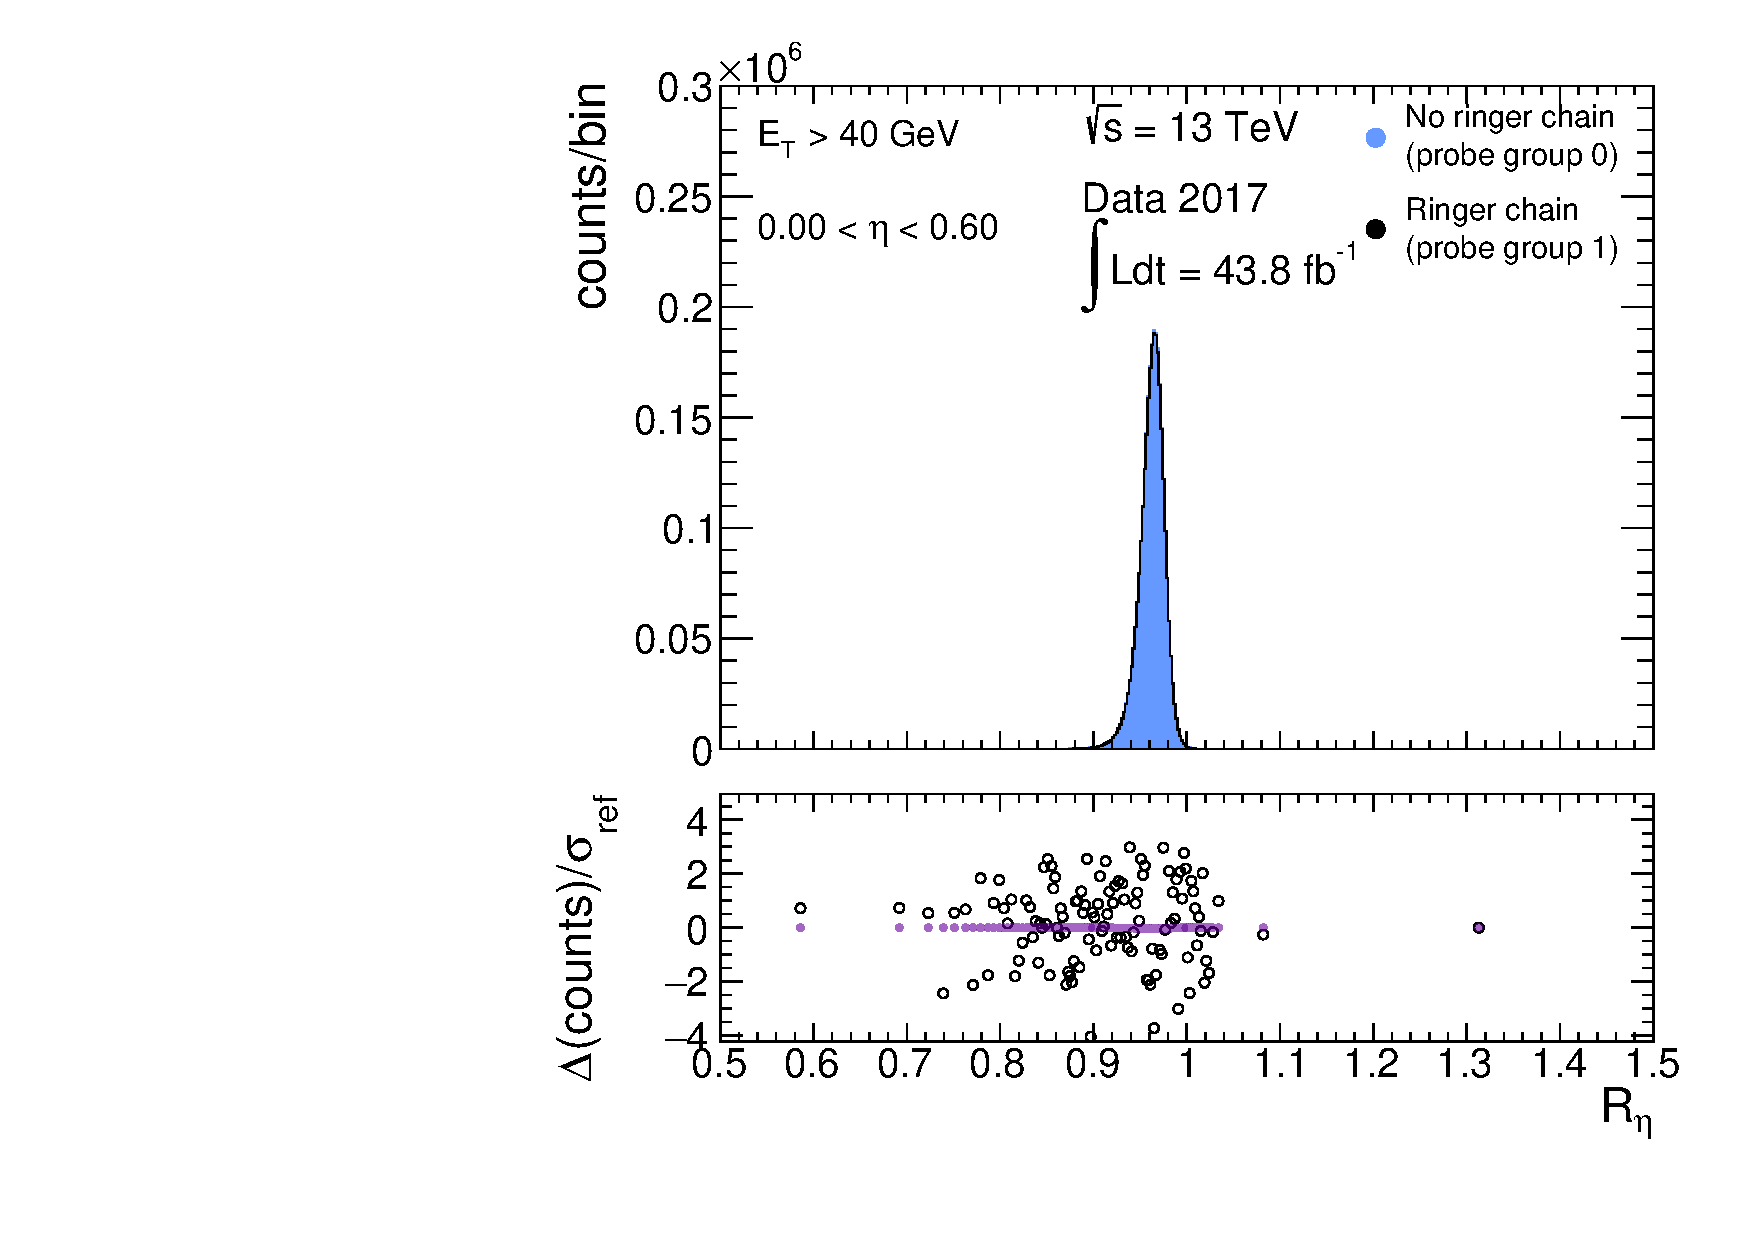
\includegraphics[width=\textwidth]{sections/analyses/figures/noAdjustment/el_reta_et40eta0_00_sigma_base_new.pdf}
\caption{}%

\end{subfigure}
\hfill
\begin{subfigure}[c]{.48\textwidth}
\centering
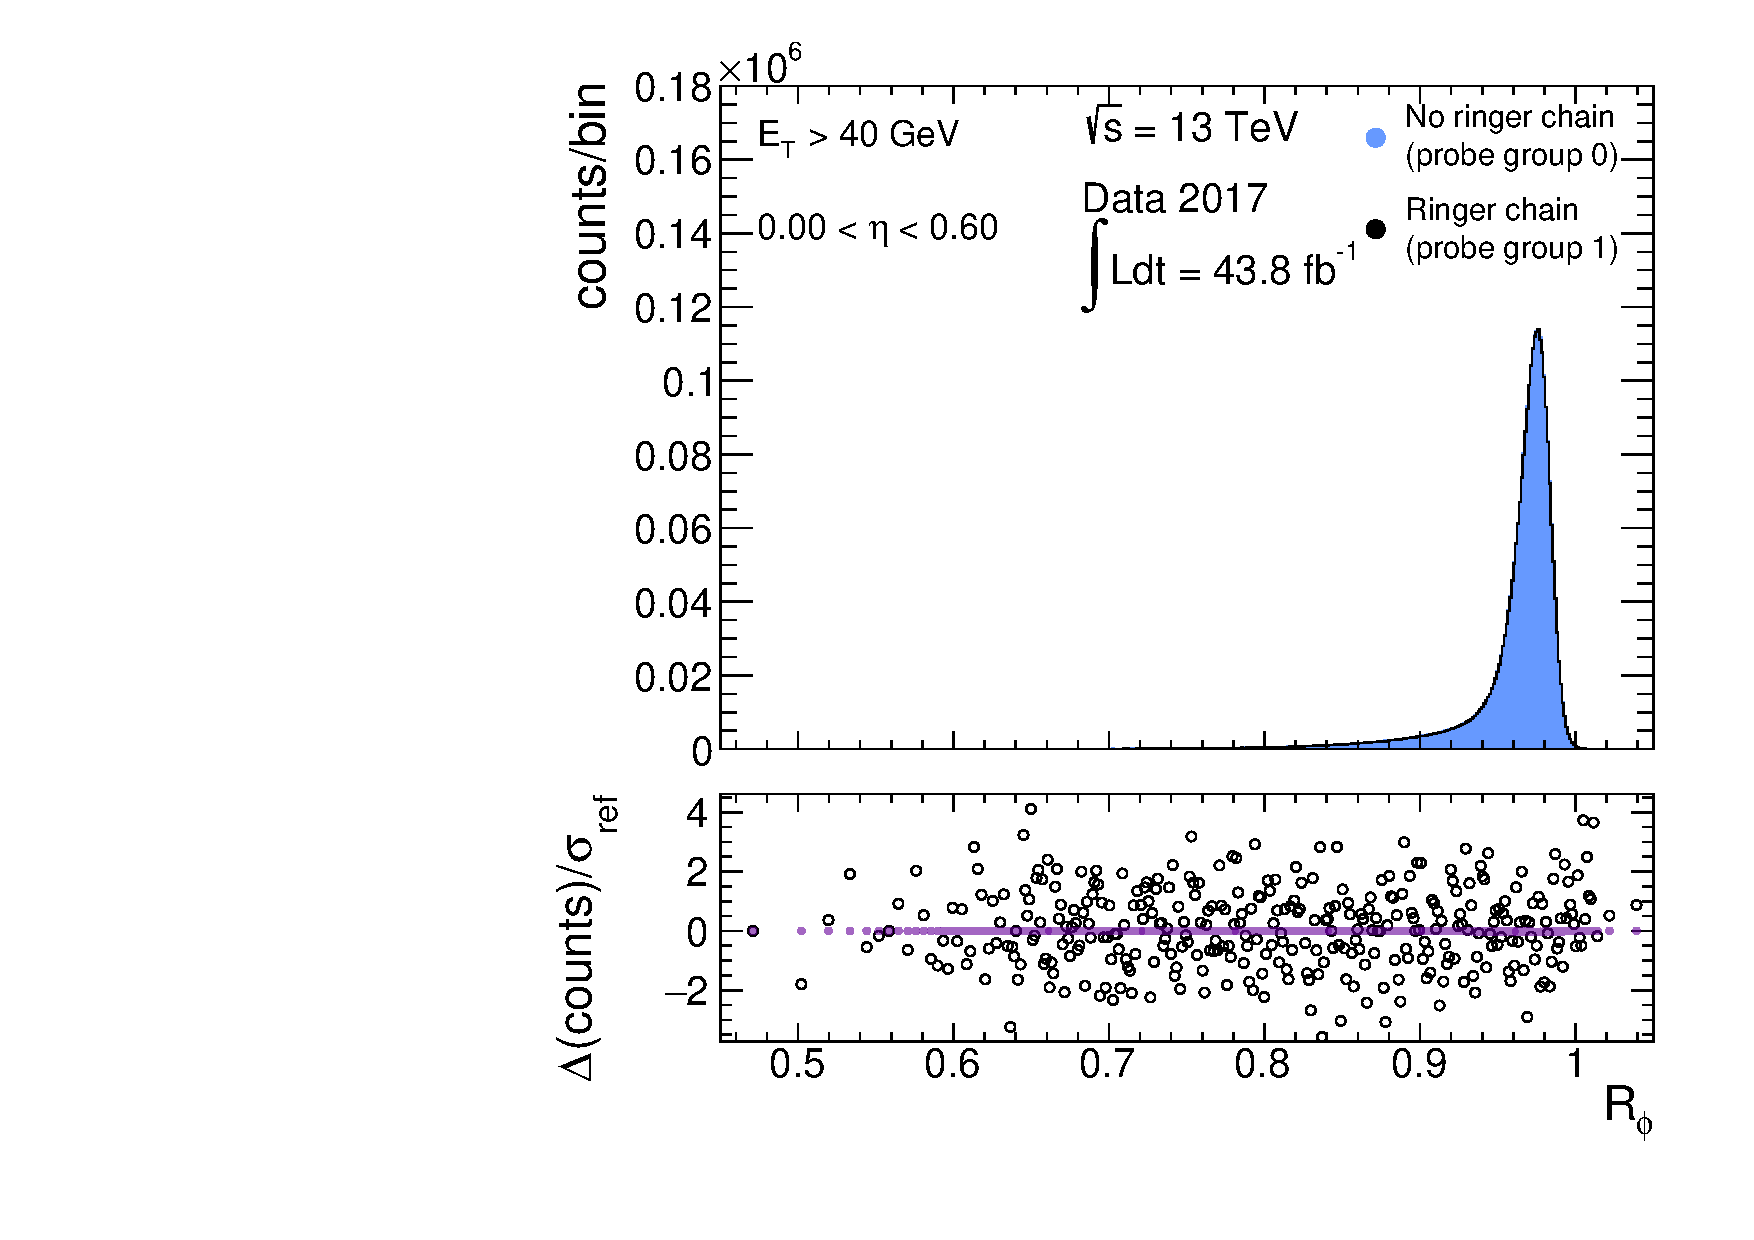
\includegraphics[width=\textwidth]{sections/analyses/figures/noAdjustment/el_rphi_et40eta0_00_sigma_base_new.pdf}
\caption{}%

\end{subfigure} \\
\begin{subfigure}[c]{.48\textwidth}
\centering
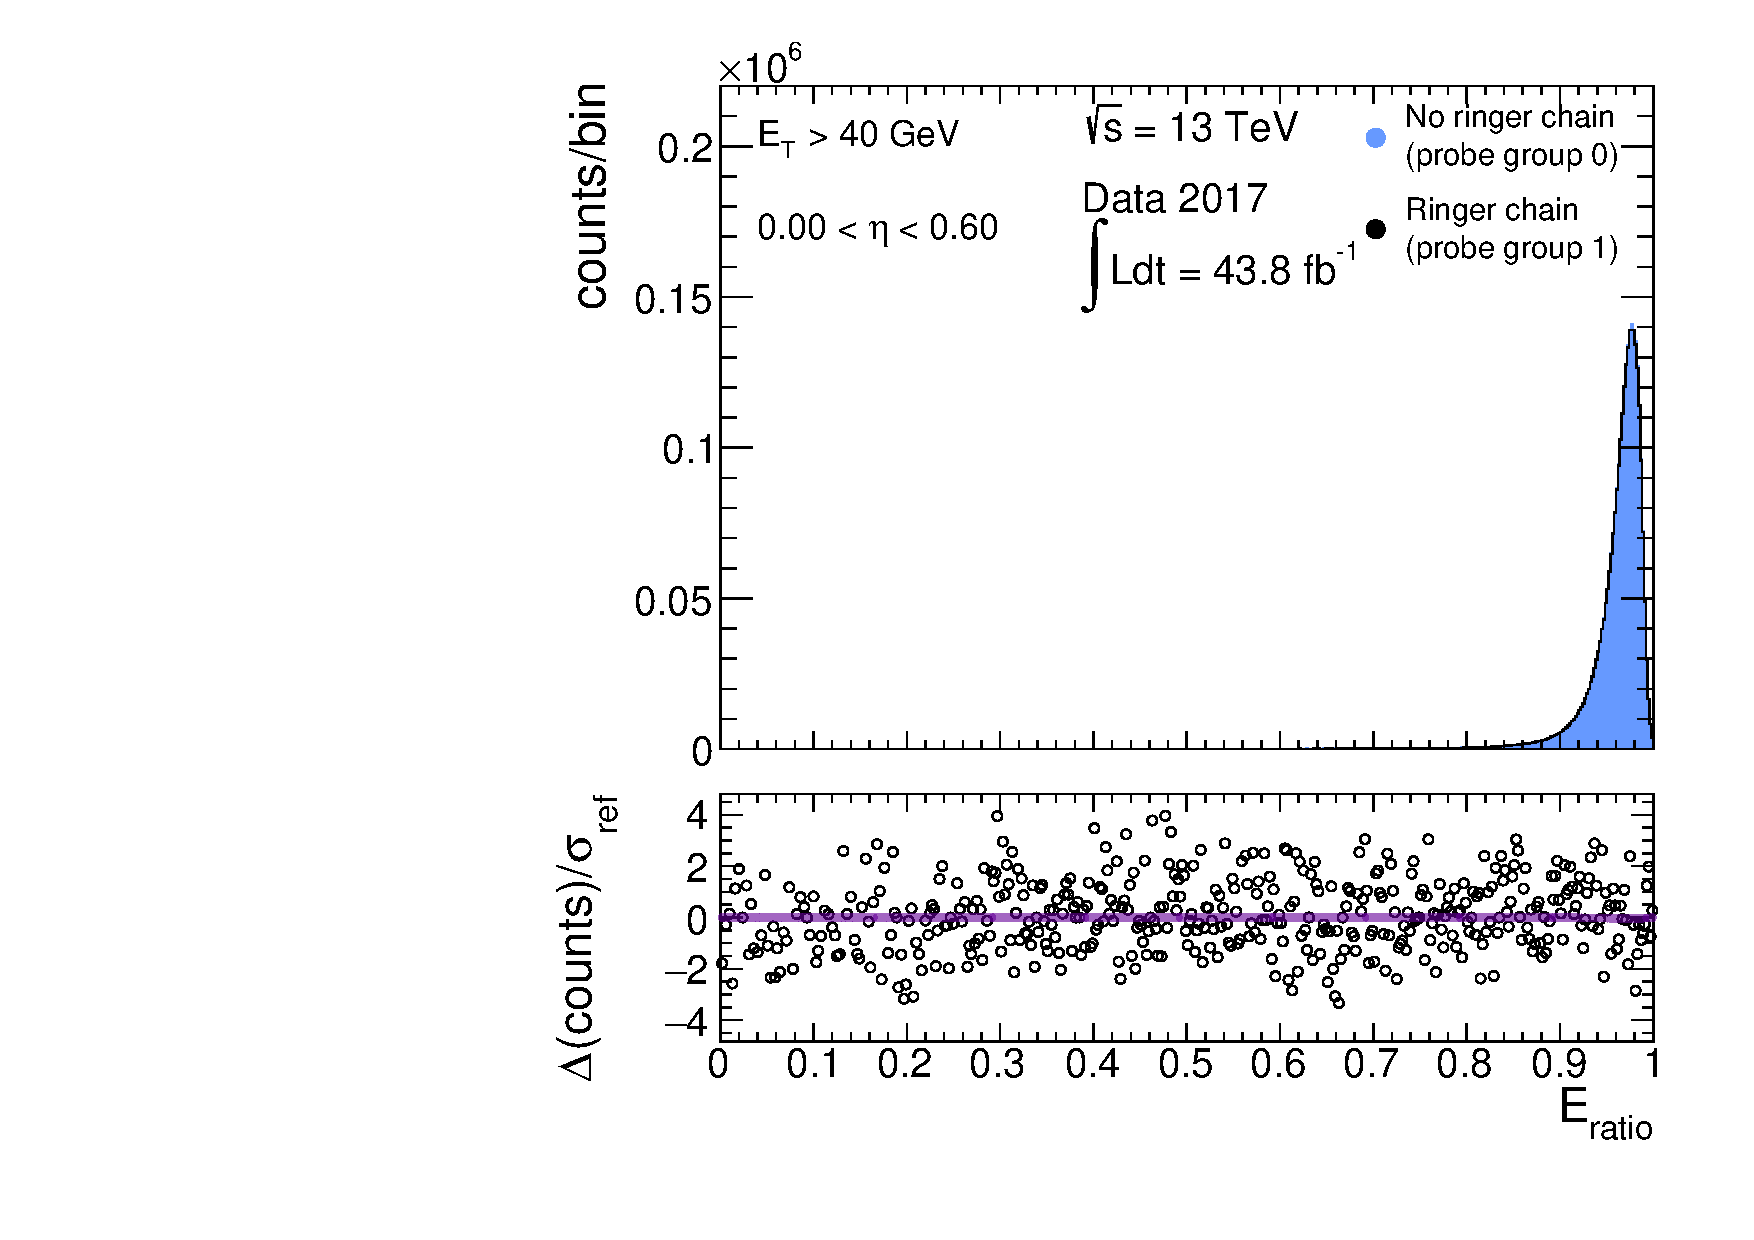
\includegraphics[width=\textwidth]{sections/analyses/figures/noAdjustment/el_eratio_et40eta0_00_sigma_base_new.pdf}
\caption{}%

\end{subfigure}
\hfill
\begin{subfigure}[c]{.48\textwidth}
\centering
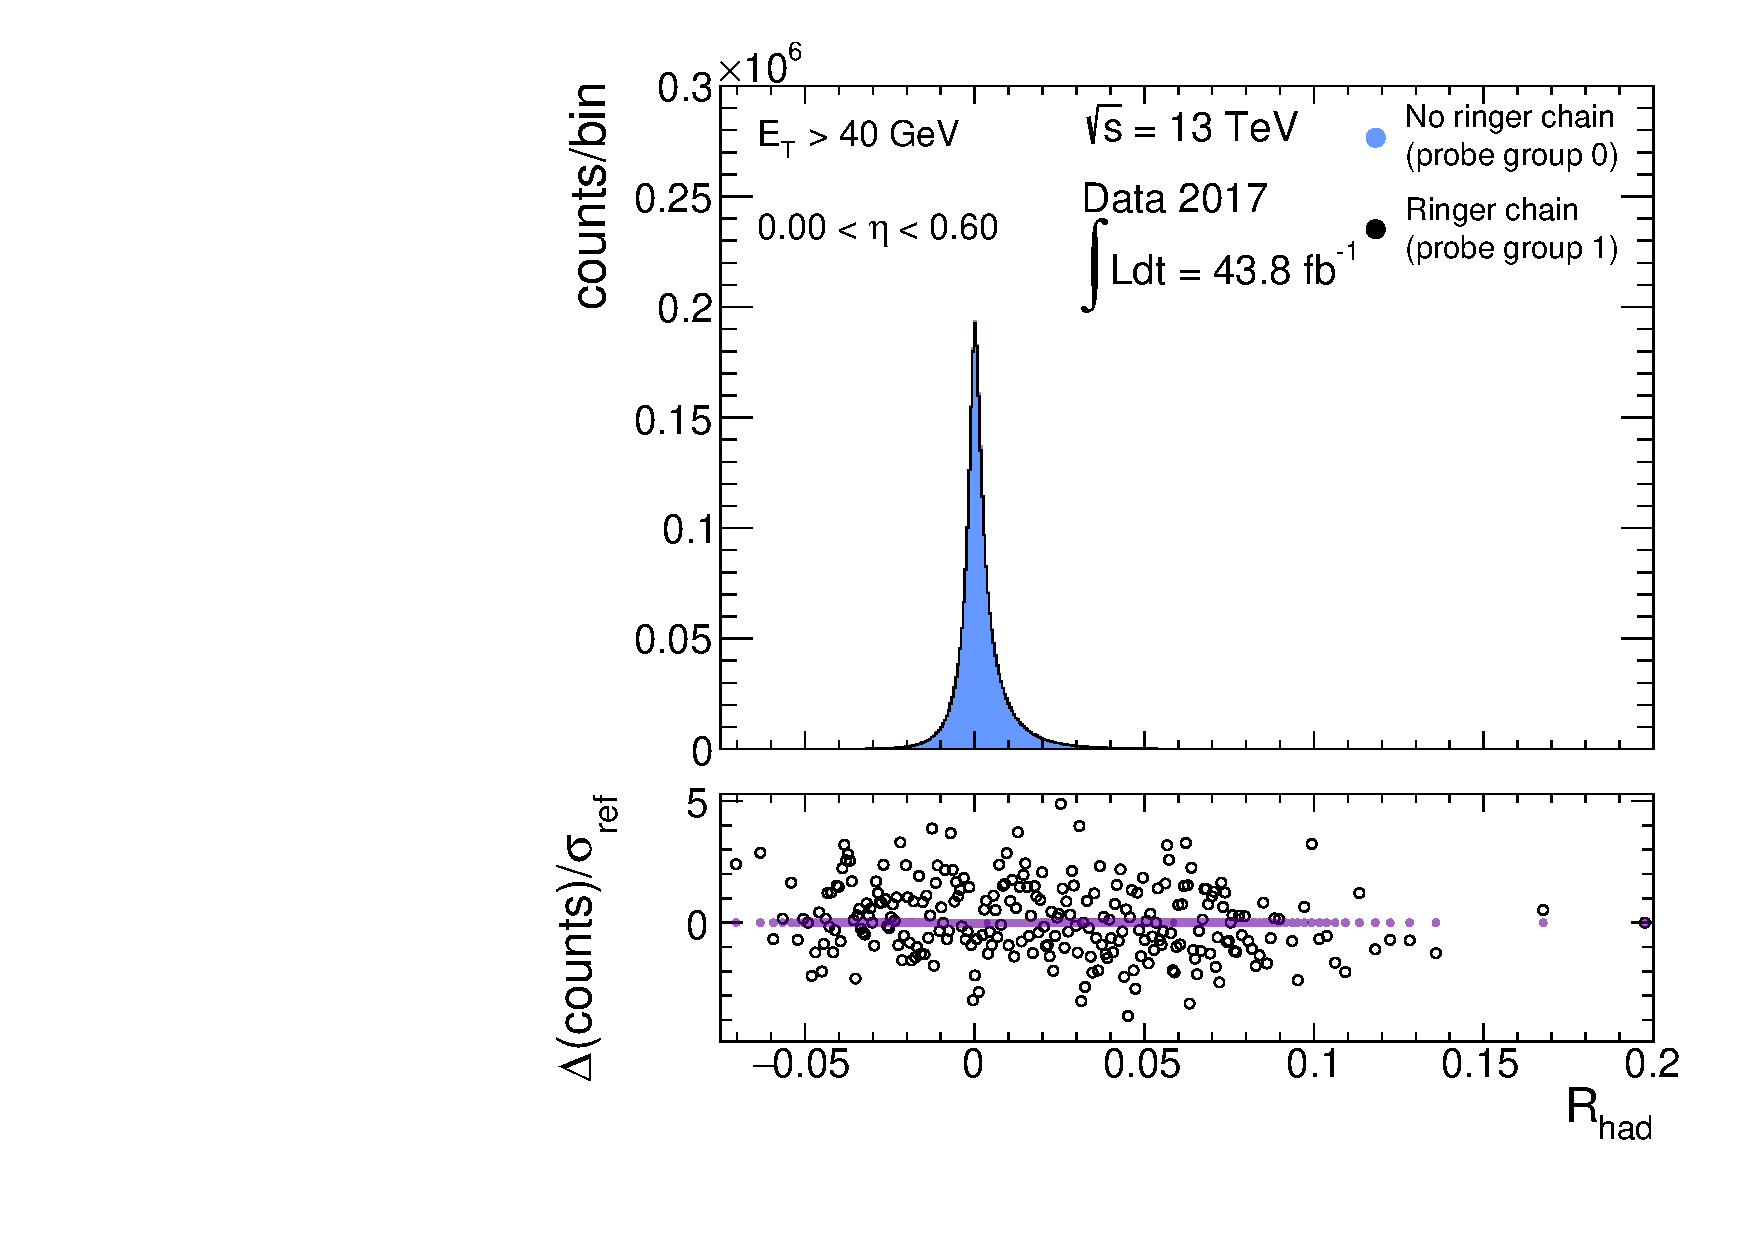
\includegraphics[width=\textwidth]{sections/analyses/figures/noAdjustment/el_rhad_et40eta0_00_sigma_base_new.pdf}
\caption{}%

\end{subfigure} \\
\caption{%
	Top: \reta, \eratio, \rphi, \rhad histogram profiles for the calorimetry variables employed in the offline likelihood in the $\et>\SI{40}{\GeV}$ and $0.00<\abseta{}<0.80$ regions using data collected by
	triggering without \rnn{} in the first arbitrary data group
	(blue area) and data collected by triggering with \rnn{} in the second
	arbitrary data group (black line).  Bottom: residual contributions using as
	statistics $\chi^s$ (equation~\ref{eq:signed_chi}, in black) and the expected
	model for no distortion given by the $\chi^s$ residuals w.r.t.\@ the
	reference.
}%
\label{fig:groups_homogeneity_calo}
\end{center}
\end{figure}%

% \begin{comment}

% \begin{figure}[t]%\ContinuedFloat
% \begin{center}
% \hspace*{\fill}
% \begin{subfigure}[c]{.48\textwidth}
% \centering
% 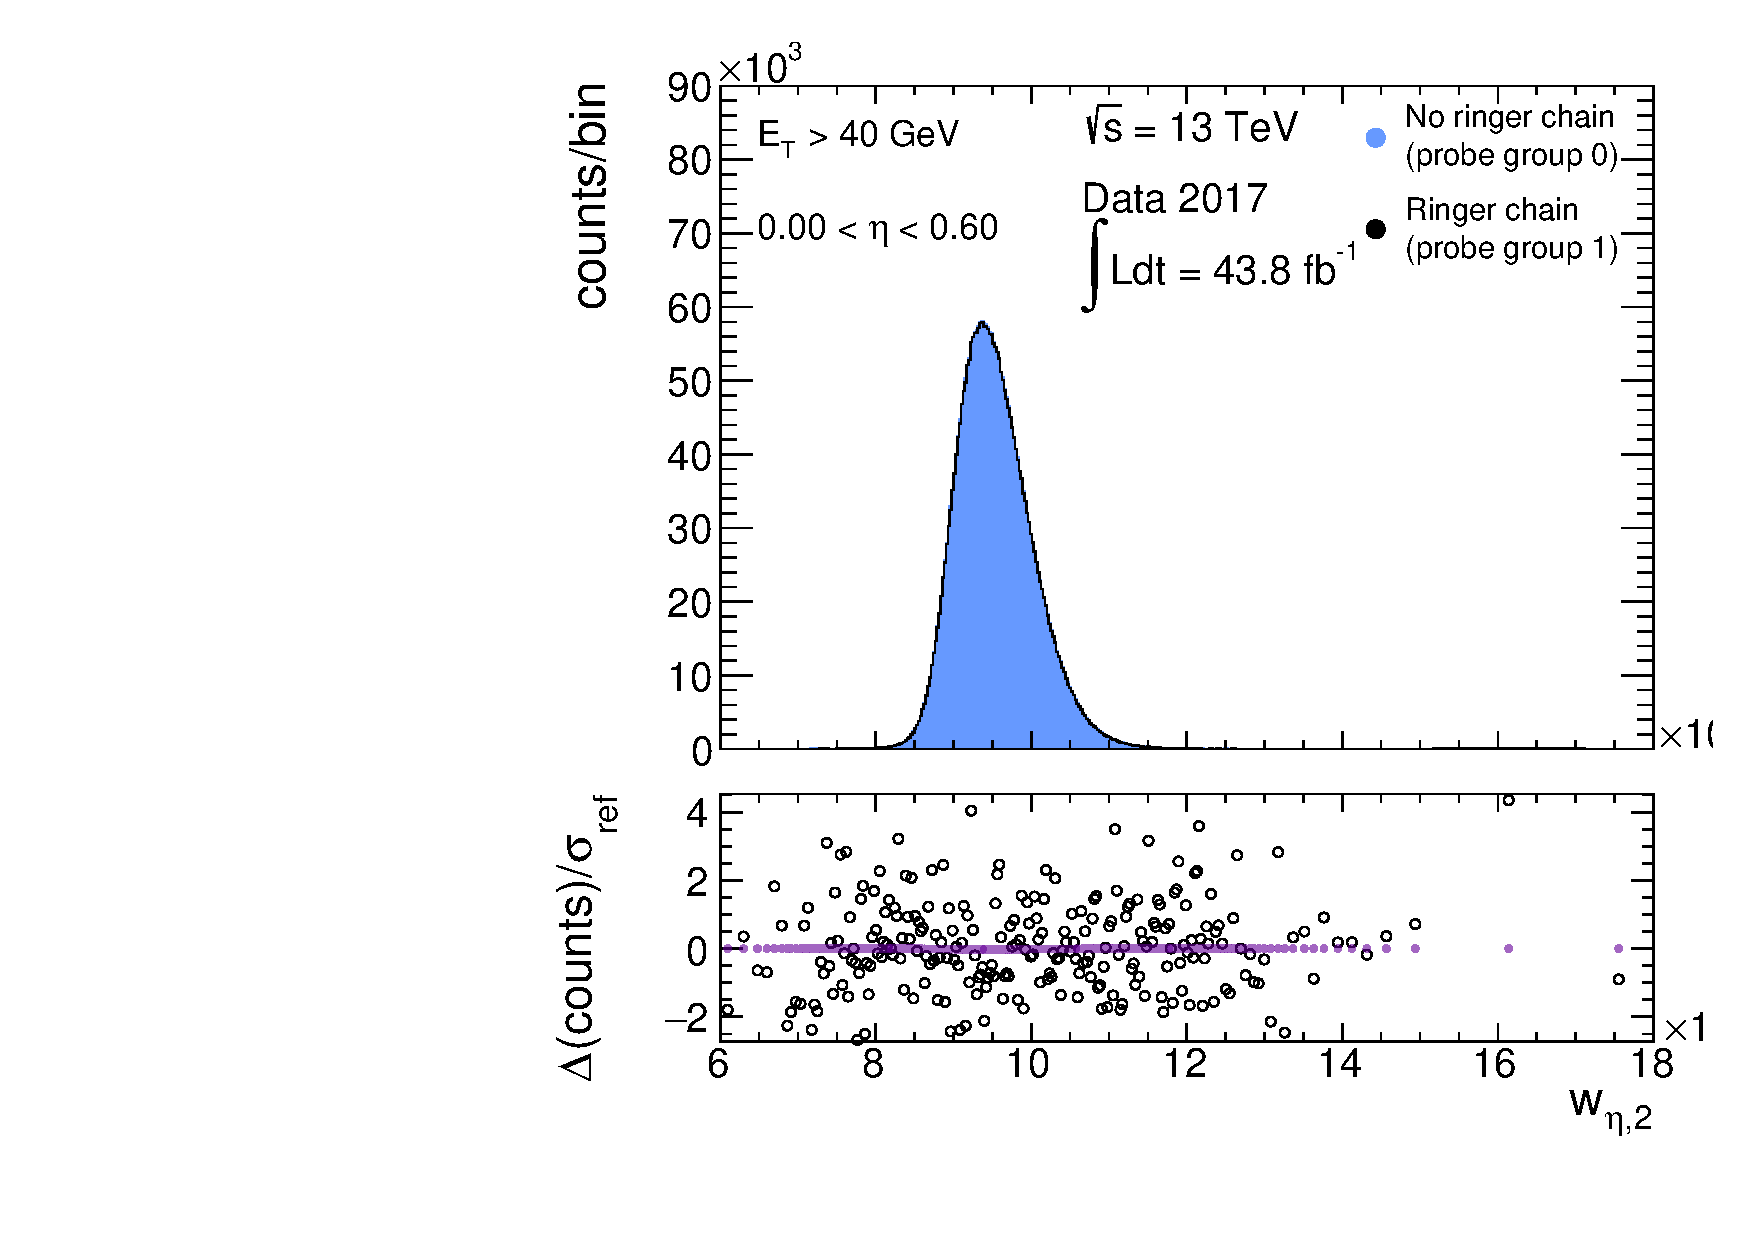
\includegraphics[width=\textwidth]{sections/analyses/figures/noAdjustment/el_weta2_et40eta0_00_sigma_base_new.pdf}
% \caption{}%

% \end{subfigure}
% \hspace*{\fill} \\
% \begin{subfigure}[c]{.48\textwidth}
% \centering
% 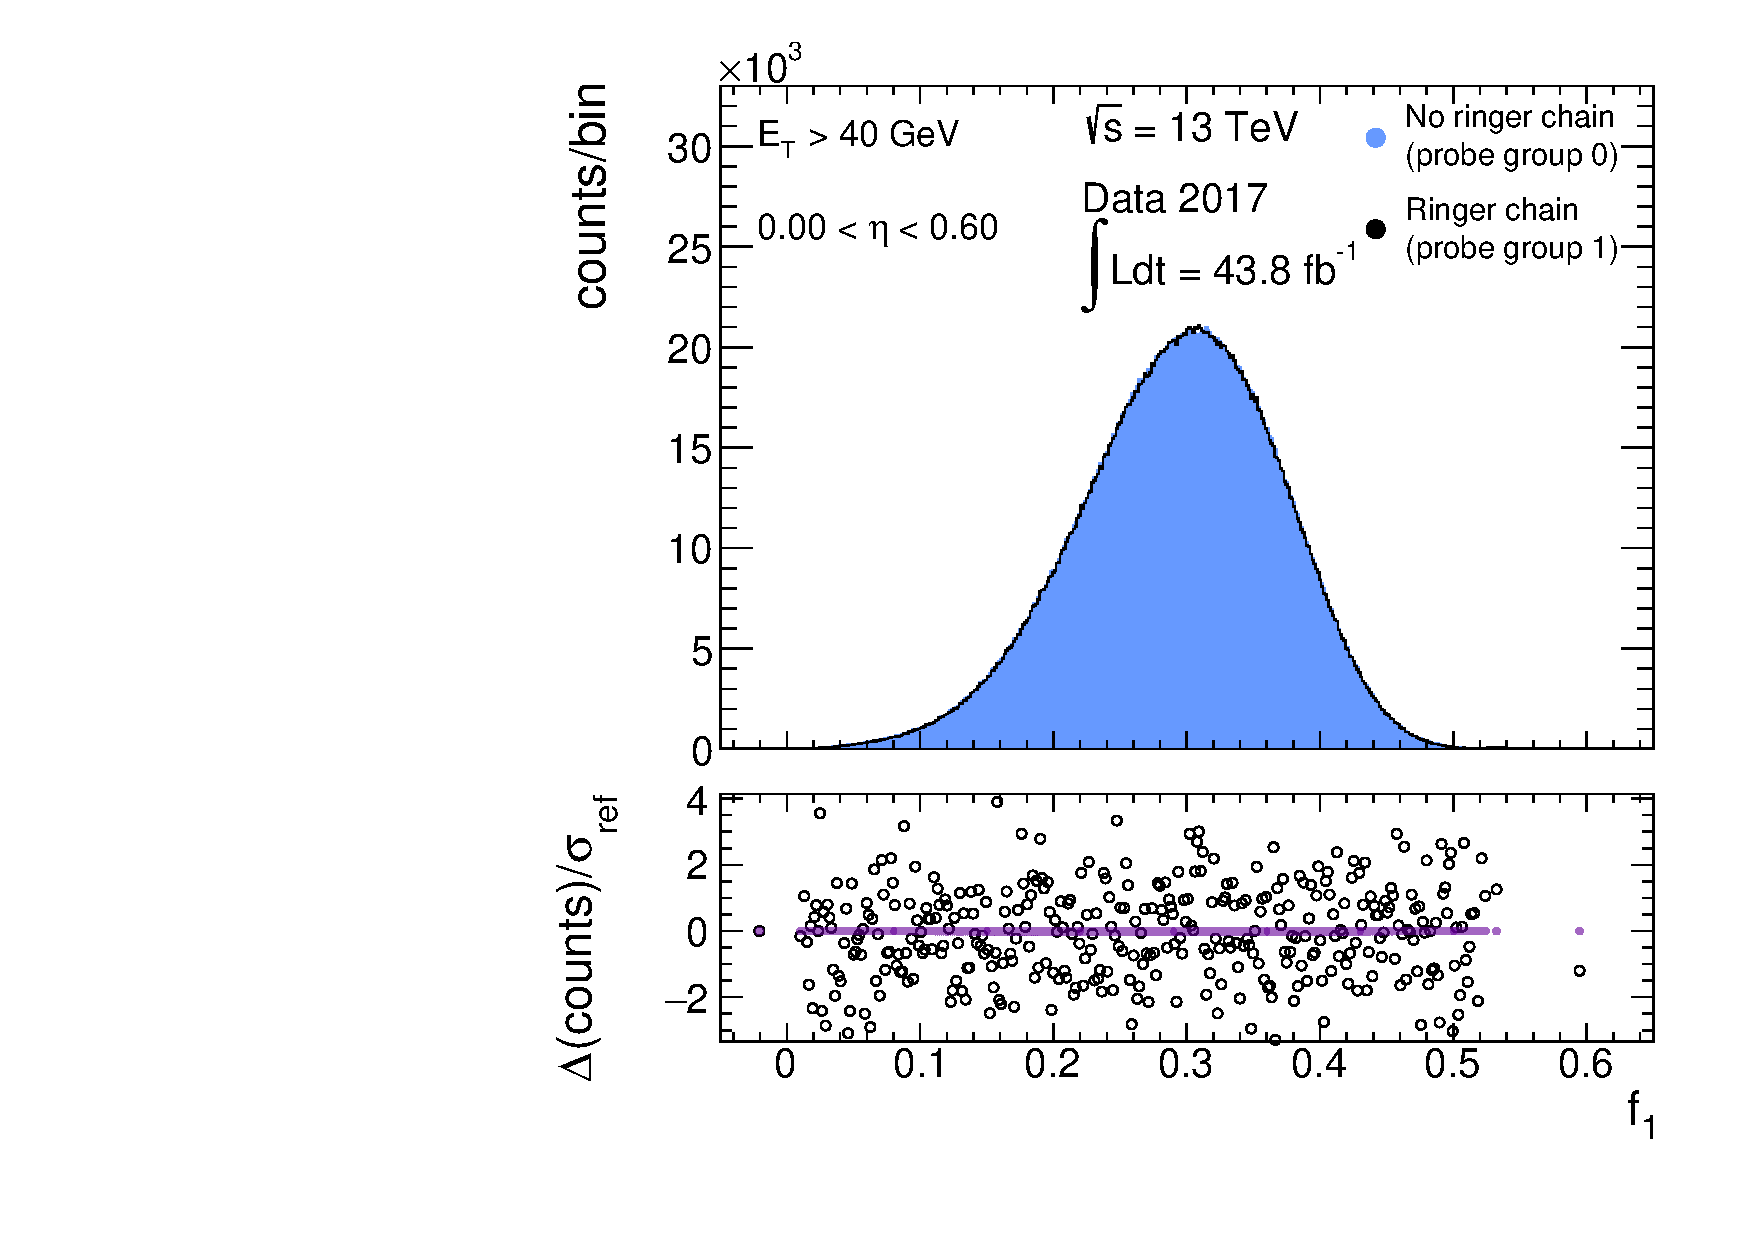
\includegraphics[width=\textwidth]{sections/analyses/figures/noAdjustment/el_f1_et40eta0_00_sigma_base_new.pdf}
% \caption{}%

% \end{subfigure}
% \hfill
% \begin{subfigure}[c]{.48\textwidth}
% \centering
% 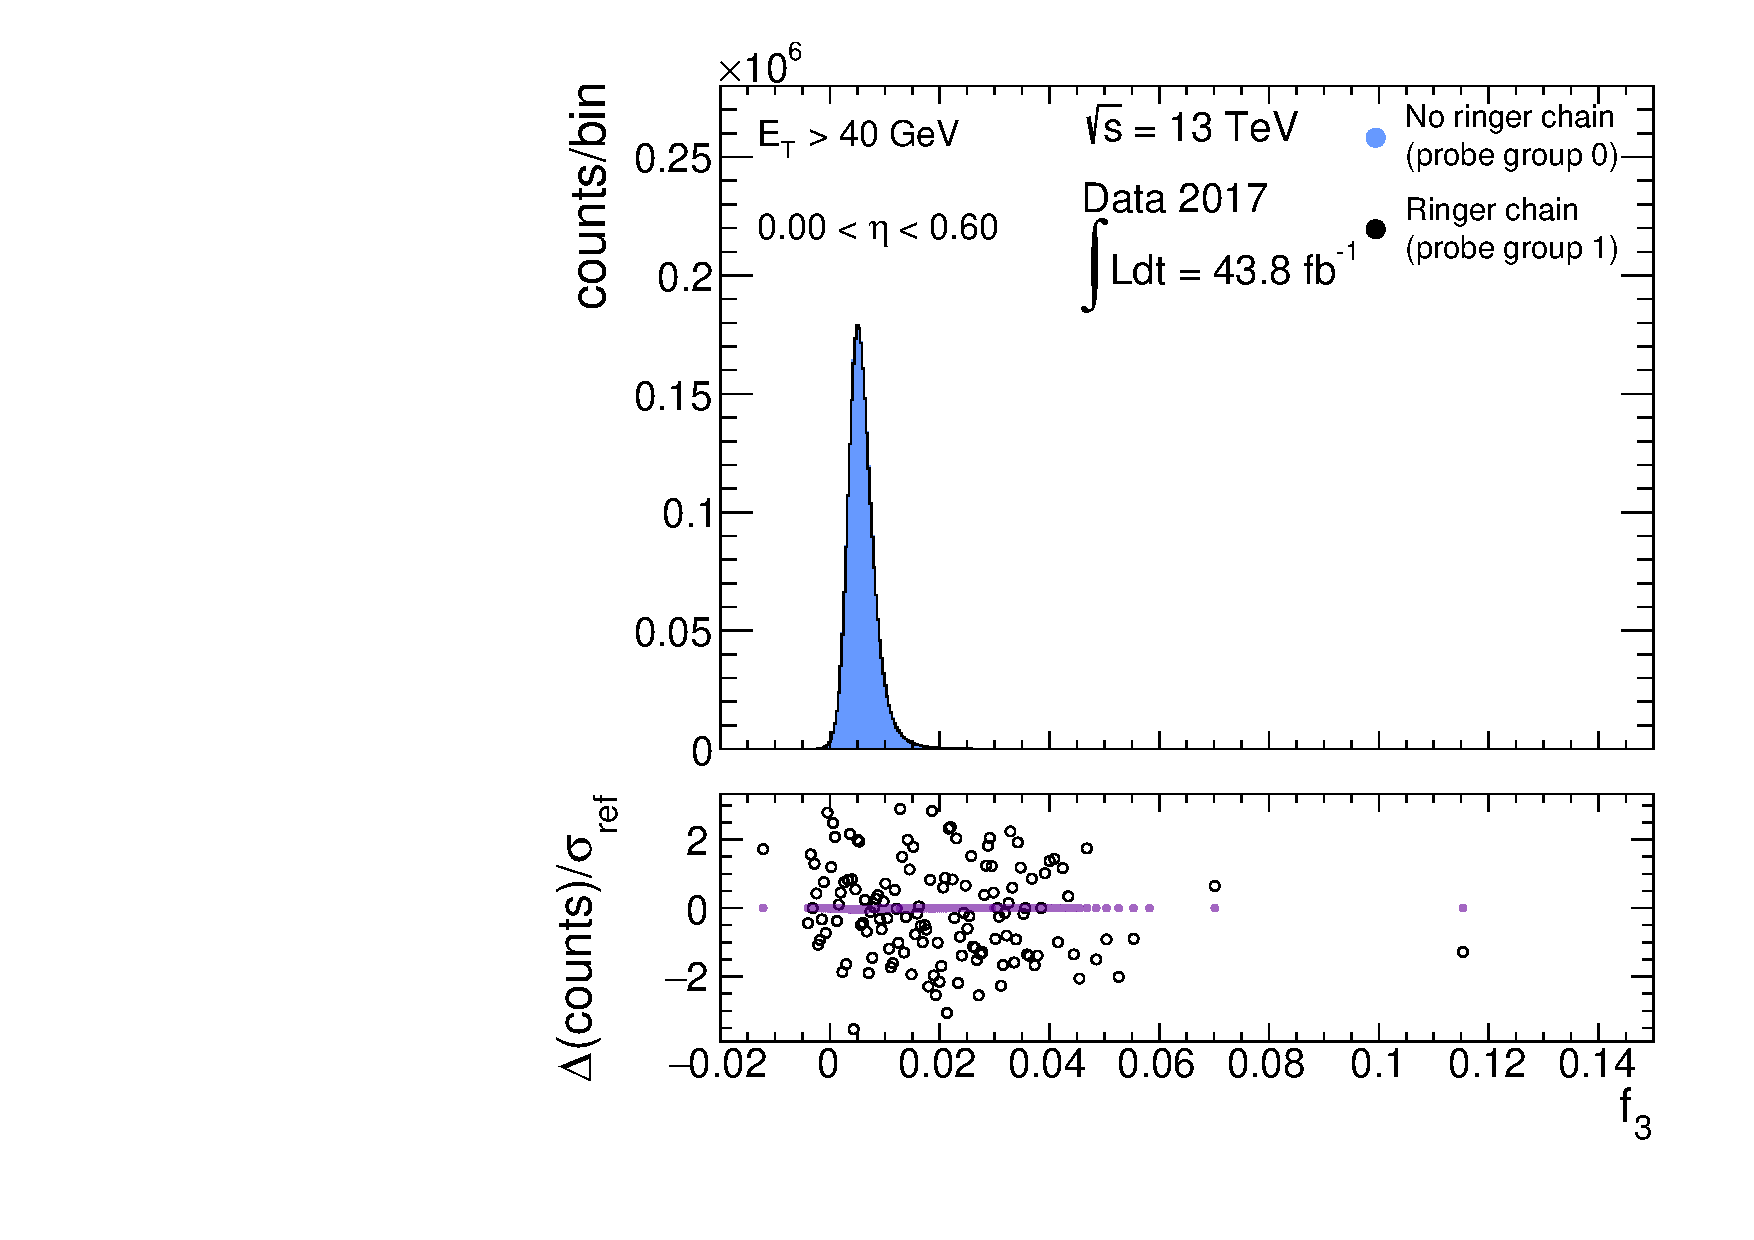
\includegraphics[width=\textwidth]{sections/analyses/figures/noAdjustment/el_f3_et40eta0_00_sigma_base_new.pdf}
% \caption{}%

% \end{subfigure} \\
% \caption{%
% Top: \weta, \fI, \fIII histogram profiles for the calorimetry variables employed in the offline likelihood in the $\et>\SI{40}{\GeV}$ and $0.00<\abseta{}<0.80$ regions using data collected by
% triggering without \rnn{} in the first arbitrary data group
% (blue area) and data collected by triggering with \rnn{} in the second
% arbitrary data group (black line).  Bottom: residual contributions using as
% statistics $\chi^s$ (equation~\ref{eq:signed_chi}, in black) and the expected
% model for no distortion given by the $\chi^s$ residuals w.r.t.\@ the
% reference.
% }%
% \label{fig:groups_homogeneity_calo_2}
% \end{center}
% \end{figure}
% \end{comment}

\FloatBarrier
